\section{Finding candidate bugs}

The first phase of analysis is to locate all of the places in the program which might exhibit a bug of the desired class.

\subsection{Formal definition of the kind of bug which we look for}
\label{sect:finding_bugs:finding_candidate_bugs:formal_definition}
For the purposes of this section, we define a bug to be a tuple $(R, W, P)$ such that:

\begin{itemize}
\item[P valid] $P$ is a sequence of dynamic instructions which form a prefix of a possible execution of the program.
\item[R valid] $R$ is a sequence of dynamic instructions in a single thread such that $P \concatDynTraces R$, where $\concatDynTraces$ is simple concatenation, is a prefix of a possible execution of the program.
\item[W valid] Similarly, $W$ is a sequence of dynamic instructions in a single thread such that $P \concatDynTraces W$ is a prefix of a possible execution of the program.
\item[R atomic] $P \concatDynTraces R$ does not crash.
\item[W atomic] $P \concatDynTraces W \concatDynTraces R$ does not crash.
\item[W isolation] $W$ does not load from any locations which are stored to by $R$.
\item[Crash possible] $P \concatDynTraces (W \interleaveDynTraces R)$ can crash, where $\interleaveDynTraces$ is the interleaving of dynamic instruction traces.
\item[Concurrent] It is possible for the program to be in state S with one thread at the first instruction of $R$ while another thread is simultaneously at the first instruction of $W$.
\end{itemize}

We assume that programs execute an infinite sequence of no-op operations before the start of the program itself.

The intuition for this is that R is an operation which reads from some
shared structure and W is an operation which updates it, and the bugs
which we're looking for are those where inadequate synchronisation
causes the read operation to crash.  The R atomic and W atomic rules
ensure that we only need to consider concurrency-related bugs (if some
behaviour is possible when the machines are run atomically then it
clearly isn't a concurrency bug).  W isolation is a somewhat
unfortunate property, and restricts the set of bugs which we can
consider in an important way, but is necessary for the analysis to be
tractable~\needCite{}.

\subsubsection{Assumptions about the program}

Big ones:

\begin{itemize}
\item
  Only need to consider two threads at a time.  This is stronger than
  just assuming that each bug only involves two threads, because a
  third thread can sometimes make a race either possible or not
  possible, and that can lead to bug hiding as $N_r$ increases.
\item
  The no-mandatory-concurrency assumption.
\end{itemize}

\subsubsection{Effect of setting the $N_r$ and $N_w$}

The set of bugs detected by SLI depends on the size of the two
analysis windows, $N_r$ and $N_w$.  Setting these to two small a value
will of course lead to bugs being missed; more subtly, increasing the
size of the window can also sometimes lead to the set of bugs which is
reported shrinking.  This happens when the program depends on a
certain minimum level of concurrency in order to achieve correctness:
SLI assumes that the program does not crash if all of the instructions
in the analysis window are run atomically; if the program requires
some minimum level of interleaving this assumption can be violated for
some interesting executions, and enlarging the analysis window will
make the problem worse.

\begin{figure}
\begin{tabular}{ll}
Read thread:         & Write thread: \\
\\
Load $t$ from loc1   & Load $t'''$ from loc1 \\
Store $t$ to loc2    & Store $t'''$ to loc2 \\
Load $t'$ from loc1  & Store $t''' + 1$ to loc2 \\
Load $t''$ from loc2 & \\
Crash if $t' == t''$ & \\
\end{tabular}
\label{fig:mandatory_concurrency1}
\caption{Example of threads with mandatory concurrency.}
\end{figure}

\begin{figure}
\begin{tabular}{ll}
Read thread:          & Write thread: \\
\\
Load $t'$ from loc1   & Load $t'''$ from loc1 \\
Load $t''$ from loc2  & Store $t'''$ to loc2 \\
Crash if $t' == t''$  & Store $t''' + 1$ to loc2
\end{tabular}
\label{fig:mandatory_concurrency2}
\caption{Truncation of the example in figure~\ref{fig:mandatory_concurrency1}.}
\end{figure}

As a concrete example, consider the threads show in
figure~\ref{fig:mandatory_concurrency1}.  Running the read thread
atomically is guaranteed to crash, from any starting state, and so
there will be no valid bug tuples based on the complete definition of
these threads.  On the other hand, if the read thread is truncated as
shown in figure~\ref{fig:mandatory_concurrency2} then there may be
such a tuple:

\begin{itemize}
\item The R atomic rule is satisfied provided that the initial value of loc1 is not equal to loc2.
\item The W atomic rule is satisfied by any initial state.
\item The concurrent rule is satisfied by this crashing interleaving:
  \begin{itemize}
  \item Load $t'$ from loc1
  \item Load $t'''$ from loc1
  \item Store $t'''$ to loc2
  \item Load $t''$ from loc2
  \item Crash if $t' == t''$
  \end{itemize}
\end{itemize}

In this particular case, the crashing execution is far more likely
than the non-crashing one even when the threads are being run in
parallel and so it is highly unlikely that this precise behaviour
would be found in a real program.  On the other hand, if there were a
large amount of code between the final two load operations in the
final thread then it might make the surviving interleaving unlikely.
This is not generally an issue for SLI, as introducing enough extra
instructions to ensure that behaviour would generally push the first
load out of the analysis window so that SLI never sees the confusing
behaviour.  This means that, for most practical purposes, the set of
bugs found by increases monotonically with the size of the analysis
window, which in turn means that a very simple heuristic suffices for
setting the size of the window: use the largest window which allows
the analysis to complete in an acceptable amount of time.

\todo{It'd be nice to have some evidence of that.}

A more powerful analysis framework might be able to increase the
window size sufficiently that the first part of the read thread would
not ``fall out''.  Even in that case, the monotonicity property would
probably still hold for most realistic programs.  The fundamental
problem here is one of mandatory concurrency: in the larger program,
running the read thread in isolation is guaranteed to crash, but it
can be ``rescued'' by being interleaved with the write thread.  The
bug here is caused by insufficient concurrency, but SLI is only
capable of handling bugs caused by excessive concurrency.
Excess-concurrency bugs are far more common than
insufficient-concurrency bugs, for several reasons:

\begin{itemize}
\item
  An insufficient-concurrency bug indicates that the programmer got
  the sequential case wrong but the concurrent case correct.  The
  concurrent case is usually far more difficult to design and reason
  about than the sequential one, and so this is an unusual
  outcome\needCite{}.
\item
  The sequential case generally receives more testing than the
  concurrent one, simply as an artifact of the way most test cases are
  constructed\needCite{}.
\item
  For most programs, there are far more concurrent executions than
  sequential ones, and so it is more likely that there are errors on
  an untested concurrent path than that there are errors on an
  untested sequential one.
\end{itemize}

SLI therefore completely ignores these insufficient-concurrency bugs.

\todo{Mention something about finding a bunch of
  insufficient-concurrency bugs related to malloc() failure?}

\begin{figure}
Illustration of a bug tuple.  We have a prefix P, write section W, and read section R.
\label{fig:mandatory_concurrency3}
\end{figure}

I now show that insufficient-concurrency bugs are the only case in
which the monotonicity property might be violated.  To see this,
consider execution shown in figure~\ref{fig:mandatory_concurrency3}.
Suppose that this execution does not generate a bug tuple.  Then
moving an instruction from $R$ or $W$ into $P$ also cannot generate a
bug tuple, and so by induction no smaller analysis windows can
generate bug tuples.

From the fact that larger windows do not generate bug tuples, we know
that:

\begin{itemize}
\item $P \concatDynTraces R \not= \survive$, from the R atomic rule, or
\item $P \concatDynTraces W \concatDynTraces R \not= \survive$, from the W atomic rule, or
\item $\crash \notin P \concatDynTraces (R \interleaveDynTraces W)$, from the concurrent rule.
\end{itemize}

Define $W = w \concatDynTraces W'$ and $R = r \concatDynTraces R'$, so
that $w$ is the first instruction of $W$ and $W'$ all the others, and
likewise for $r$, $R$, and $R'$.  Shrinking the analysis window then
corresponds to replacing $R$ with $R'$ and $P$ with $P
\concatDynTraces r$, or replacing $W$ with $W'$ and $P$ with $P
\concatDynTraces w$.  We therefore generate a bug tuple with the
reduced window if:

\begin{align*}
( & (P \concatDynTraces w \concatDynTraces R & = & \survive) & \wedge \\
  & (P \concatDynTraces W \concatDynTraces R & = & \survive) & \wedge \\
  & ((P \concatDynTraces w \concatDynTraces (R \interleaveDynTraces W')) & \ni & \crash)) & \vee \\
( & (P \concatDynTraces R & = & \survive) & \wedge \\
  & (P \concatDynTraces r \concatDynTraces W \concatDynTraces R' & = & \survive) & \wedge \\
  & ((P \concatDynTraces r \concatDynTraces (R' \interleaveDynTraces W)) & \ni & \crash))
\end{align*}

Combining those together, we find that reducing the analysis window can introduce a new bug if:

\begin{align*}
( & (P \concatDynTraces R & \not= & \survive) & \wedge \\
  & (P \concatDynTraces W \concatDynTraces R & \not= & \survive) & \wedge \\
  & ((P \concatDynTraces (R \interleaveDynTraces W)) & \not{}\ni & \crash)) & \vee \\
( & (P \concatDynTraces w \concatDynTraces R & = & \survive) & \wedge \\
  & (P \concatDynTraces W \concatDynTraces R & = & \survive) & \wedge \\
  & ((P \concatDynTraces w \concatDynTraces (R \interleaveDynTraces W')) & \ni & \crash)) & \vee \\
( & (P \concatDynTraces R & = & \survive) & \wedge \\
  & (P \concatDynTraces r \concatDynTraces W \concatDynTraces R' & = & \survive) & \wedge \\
  & ((P \concatDynTraces r \concatDynTraces (R' \interleaveDynTraces W)) & \ni & \crash))
\end{align*}

Simple boolean algebra, plus the obvious rule that $P \concatDynTraces (R \interleaveDynTraces W) = (P \concatDynTraces r \concatDynTraces (R' \interleaveDynTraces W) ) \cup (P \concatDynTraces w \concatDynTraces (R \interleaveDynTraces W') ) $, reduces that to this:

\begin{align*}
( & (P \concatDynTraces r \concatDynTraces R' & = & \crash) & \wedge \\
  & (P \concatDynTraces w \concatDynTraces r \concatDynTraces R' & = & \survive) & \wedge \\
  & (P \concatDynTraces w \concatDynTraces W' \concatDynTraces r \concatDynTraces R' & = & \survive) & \wedge \\
  & ((P \concatDynTraces w \concatDynTraces (W' \interleaveDynTraces R)) & \ni & \crash)) & \vee \\
( & (P \concatDynTraces r \concatDynTraces R' & = & \survive) & \wedge \\
  & (P \concatDynTraces w \concatDynTraces W' \concatDynTraces r \concatDynTraces R' & = & \crash) & \wedge \\
  & (P \concatDynTraces w \concatDynTraces r \concatDynTraces R' & = & \survive) & \wedge \\
  & (P \concatDynTraces r \concatDynTraces w \concatDynTraces W' \concatDynTraces R' & = & \survive) & \wedge \\
  & ((P \concatDynTraces r \concatDynTraces (W \interleaveDynTraces R')) & \ni & \crash))
\end{align*}

Consider the first clause of the disjunction first, and in particular consider these two terms:

\begin{align*}
 & (P \concatDynTraces r \concatDynTraces R' & = & \crash) & \wedge \\
 & (P \concatDynTraces w \concatDynTraces r \concatDynTraces R' & = & \survive)
\end{align*}

The definition of crash used in SLI is that the final instruction of $R'$ crashes, and so adding further instructions after that point cannot possible change the result.
Those terms are therefore equivalent to these:

\begin{align*}
 & (P \concatDynTraces r \concatDynTraces R' \concatDynTraces w \concatDynTraces W' & = & \crash) & \wedge \\
 & (P \concatDynTraces w \concatDynTraces r \concatDynTraces R' \concatDynTraces W' & = & \survive)
\end{align*}

In other words, $R$ is doomed when run in isolation, but running it in parallel with $W$ can save it.
That is precisely the definition of mandatory concurrency used above.

Consider the second clause now.
That contains these two terms:

\begin{align*}
  & (P \concatDynTraces w \concatDynTraces W' \concatDynTraces r \concatDynTraces R' & = & \crash) & \wedge \\
  & (P \concatDynTraces r \concatDynTraces w \concatDynTraces W' \concatDynTraces R' & = & \survive)
\end{align*}

This is even more clear: running $W$ and then $R$ atomically leads to a crash, but allowing $W$ to interrupt $R$ saves the execution.
Once again, this clause is only satisfiable in the presence of mandatory concurrency.

Therefore, it is only possible for shrinking the analysis window to reveal more bugs in the presence of mandatory concurrency, and, conversely, when the program does not use mandatory concurrency, enlarging the analysis window cannot disguise bugs.
This monotonicity property is useful because it provides a simple rule for setting the size of the analysis window: use the largest such that the analysis completes in a reasonable amount of time.
There is no need for the user to carefully select a window size for their program, or to try multiple window sizes in order to reveal additional bugs.

\label{sect:monotonicity}

\todo{This proof feels quite circular and unconvincing.  May need more thought here.}

\subsection{Crash summaries}

This analysis produces a series of crash summaries.
Each summary represents a (possibly infinite) set of bug tuples has several components:

\begin{itemize}
\item The read \StateMachine, corresponding to the $R$ member of the bug tuple.
\item The write \StateMachine, corresponding to the $W$ member of the bug tuple.
\item The verification condition, a predicate on the program's state which corresponds to the $S$ member of the bug tuple.
\item An aliasing table, which says which memory-accessing instructions in the read and write \StateMachines might access the same area of memory.
\end{itemize}

A crash summary represents a bug tuple $(R, W, S)$ if the summary's read \StateMachine includes the dynamic instruction trace $R$, its write \StateMachine includes the dynamic instruction trace $W$, and the verification condition is true of $S$.
The set of summaries produced by the analysis is defined to be complete if every possible bug tuple is represented by at least one crash summary, and sound if the crash summaries only represent valid bug tuples.
The analysis presented here is, in that sense, complete, subject to some caveats discussed in later sections, but not sound.

\section{\STateMachines}

The \StateMachines themselves consist of three components:

\begin{itemize}
\item
  A slice of the program in a simple analysis language.  Programs in
  this language consist of a directed acyclic graph of analysis
  states.  The states fall into one of three classes: terminals, with
  no successors; side-effects, with a single successor; or choices,
  with two successors.  The side-effects can express obvious
  program-level effects such as accessing memory or setting a
  particular register, but also less-obvious ones such as register
  aliasing configurations or restrictions on the set of program states
  which must be considered by later analysis steps.  Similarly, the
  expression language used for the conditions in choice states or the
  addresses for memory accessing side-effects can refer to simple
  things like the values of processor registers or the initial
  contents of memory, and can also express queries about the program's
  control flow or the happens-before graph.
\item
  A fragment of the original program's control-flow graph, covering
  all of the instructions from which the \StateMachine was generated.
  This fragment is unrolled so that each dynamic instruction in the
  analysis window is represented by precisely on node in the
  CFG\editorial{I should really try to explain what that means in a
    bit more detail.}.  Functions are inlined.  This graph fragment
  will not always be completely weakly connected if, for instance, the
  \StateMachine represents activity in multiple concurrent threads.
\item
  A table mapping memory access identifiers to sets of nodes in the
  control flow graph. \todo{Screw it; these are a pain to describe and
    they're not all that important; drop them.}
\end{itemize}

\begin{figure}
  \begin{minipage}{50mm}
    \begin{subfloat}
      \begin{minipage}{50mm}
\begin{verbatim}
400694: mov    global_ptr,%rax
40069b: test   %rax,%rax
40069e: je     4006ad
4006a0: mov    global_ptr,%rax
4006a7: movl   $0x5,(%rax)
\end{verbatim}
      \end{minipage}
      \caption{Program code}
    \end{subfloat}
    \vspace{50pt}
    \begin{subfloat}
      \hspace{20mm}
      \begin{tikzpicture}
        \node (cfg6) at (0,2) [CfgInstr] {cfg6:400694};
        \node (cfg5) [CfgInstr, below=of cfg6] {cfg5:40069b};
        \node (cfg4) [CfgInstr, below=of cfg5] {cfg4:40069e};
        \node (cfg3) [CfgInstr, below=of cfg4] {cfg3:4006a0};
        \draw[->] (cfg6) -- (cfg5);
        \draw[->] (cfg5) -- (cfg4);
        \draw[->] (cfg4) -- (cfg3);
      \end{tikzpicture}
      \caption{Control-flow graph fragment}
    \end{subfloat}
  \end{minipage}
  \begin{subfloat}
    \begin{minipage}{30mm}
      \begin{tikzpicture}
        \node (l1) at (0,2) [stateSideEffect] {l1: LOAD tmp1 $\leftarrow$ global\_ptr AT cfg6 };
        \node (l2) [stateIf, below=of l1] {l2: if (0 == tmp1)};
        \node (l4) [stateSideEffect, below=of l2] {l4: LOAD tmp2 $\leftarrow$ global\_ptr AT cfg3 };
        \node (l3) [stateTerminal, right=of l4] {l3: survive};
        \node (l5) [stateIf, below=of l4] {l5: if (BadPtr(tmp2))};
        \node (l6) [stateTerminal, below=of l5] {l6: crash};
        \draw[->] (l1) -- (l2);
        \draw[->] (l2) -- node [above] { true } (l3);
        \draw[->] (l2) -- node [left] { false } (l4);
        \draw[->] (l4) -- (l5);
        \draw[->] (l5) -- node [below] { false } (l3);
        \draw[->] (l5) -- node [left] { true } (l6);
      \end{tikzpicture}
    \end{minipage}
    \caption{\STateMachine}
  \end{subfloat}
  \label{fig:intro:single_threaded_machine}
  \caption{A fragment of machine code, and the \StateMachine generated
    for a bug which leads to a crash at 4006a7.}
\end{figure}

Figure~\ref{fig:intro:single_threaded_machine} shows an example of a
simple single-threaded \StateMachine\footnote{This is the read-side of
  the simple\_toctou test in \S\ref{sect:eval:art:simple_toctou}.}.
It illustrates a simple time-of-check, time-of-use race: the program
loads from \verb|global_ptr| twice in quick succession, validating the
result of the first and using the result of the second.  The
translation to a \StateMachine is hopefully reasonably clear: the
control-flow graph covers on the left all of the relevant instructions
and the flow chart on the right expresses the relevant part of their
behaviour.  It is trivial to read off from these diagrams that the
program might crash if some other thread modifies \verb|global_ptr| in
between the two loads and will otherwise survive.

\begin{figure}
  \begin{minipage}{50mm}
    \begin{subfloat}
      \begin{minipage}{50mm}
\begin{verbatim}
4008fb: movq   $0x0,global_ptr
\end{verbatim}
      \end{minipage}
      \caption{Program code}
    \end{subfloat}
    \vspace{50pt}
    \begin{subfloat}
      \hspace{20mm}
      \begin{tikzpicture}
        \node (cfg8) at (0,2) [CfgInstr] {cfg8:4008fb};
      \end{tikzpicture}
      \caption{Control-flow graph fragment}
    \end{subfloat}
  \end{minipage}
  \begin{subfloat}
    \begin{minipage}{30mm}
      \begin{tikzpicture}
        \node (l7) at (0,2) [stateSideEffect] {l7: STORE 0 $\rightarrow$ global\_ptr AT cfg8 };
      \end{tikzpicture}
    \end{minipage}
    \caption{\STateMachine}
  \end{subfloat}
  \label{fig:intro:single_threaded_machine_write}
  \caption{The other side of the race in figure~\ref{fig:intro:single_threaded_machine}.}
\end{figure}

\begin{figure}
  \begin{tikzpicture}
    \node (lA) [stateIf] { lA: if (cfg6:thread1 \happensBefore cfg7:thread2) };
    \node (l1) [stateSideEffect, below left = of lA] { l1: LOAD tmp1 $\leftarrow$ global\_ptr AT cfg6:thread1 };
    \node (l2) [stateIf, below = of l1] { l2: if (0 == tmp1) };
    \node (lD) [stateTerminal, below left = of l2] { lD: survive};
    \node (lC) [stateIf, below right = of l2] {lC:  if (cfg3:thread1 \happensBefore cfg7:thread2) };
    \node (lE) [stateSideEffect, below left = of lC] {lE: Assert $global\_ptr = global\_ptr$ };
    \node (l7a) [stateSideEffect, below = of lE] {l7a: STORE 0 $\rightarrow$ global\_ptr AT cfg8:thread2 };
    \node (l4a) [stateSideEffect, below = of l7a] {l4a: LOAD tmp2 $\leftarrow$ global\_ptr AT cfg3:thread1 };
    \node (l5a) [stateIf, below = of l4a] { l5a: if (BadPtr(tmp2)) };
    \node (lG) [stateTerminal, below = of l5b] { lG: crash };
    \node (l4b) [stateSideEffect, below right = of lC] {l4b: LOAD tmp3 $\leftarrow$ global\_ptr AT cfg3:thread1 };
    \node (l5b) [stateIf, below = of l4b] { l5: if (BadPtr(tmp3))};
    \node (lF) [stateTerminal, below right = of l5b] { lF: unreached };
    \node (lB) [stateSideEffect, below right = of lA] { lB: Assert $global\_ptr = global\_ptr$ };
    \node (l7b) [stateSideEffect, below = of lB] { l7b: STORE 0 $\rightarrow$ global\_ptr AT cfg8:thread2 };
    \draw [->] (lA) -- (l1);
    \draw [->] (lA) -- (lB);
    \draw [->] (l1) -- (l2);
    \draw [->] (l2) -- (lD);
    \draw [->] (lC) -- (lE);
    \draw [->] (lC) -- (l4b);
    \draw [->] (lE) -- (l7a);
    \draw [->] (l7a) -- (l4a);
    \draw [->] (l4a) -- (l5a);
    \draw [->] (l5a) -- (lD);
    \draw [->] (l5a) -- (lG);
    \draw [->] (l4b) -- (l5b);
    \draw [->] (l5b) -- (lD);
    \draw [->] (l5b) -- (l8);
    \draw [->] (lB) -- (l7a);
    \draw [->] (l7a) -- (l8);
  \end{tikzpicture}
  \label{fig:intro:cross_thread}
  \caption{Cross-product of the \StateMachine shown in
    figures~\ref{fig:intro:single_threaded_machine} and
    \ref{fig:intro:single_threaded_machine_write}.}
\end{figure}

\begin{figure}
  \begin{tikzpicture}
    \node (lA) [stateSideEffect] {lA: Assert $0 \not= InitMemory(global\_ptr)$ and $cfg6:thread1 \happensBefore cfg7:thread2$}
    \node (lB) [stateIf, below = of lA] {lB: if $cfg3:thread1 \happensBefore cfg7:thread2$ };
    \node (lC) [stateTerminal, below left = of lB] {lC: survive};
    \node (lD) [stateTerminal, below right = of lB] {lD: crash};
    \draw [->] (lA) -- (lB);
    \draw [->] (lB) -- (lC);
    \draw [->] (lB) -- (lD);
  \end{tikzpicture}
  \label{fig:intro:cross_thread_opt}
  \caption{\STateMachine from figure~\ref{fig:intro:cross_thread}
    after \StateMachine simplification.}
\end{figure}

\STateMachines become somewhat more interesting when they capture the
results of multiple threads.  Figure~\ref{fig:intro:cross_thread}
shows an example of a cross-thread \StateMachine.  There are a couple
of interesting features here:

\begin{itemize}
\item Several new states have been created and existing ones
  duplicated.  In particular, some memory accesses have now been
  duplicated to multiple places in the \StateMachine
\item
  $\happensBefore$ expressions.  These allow the \StateMachine to
  query the program's happens-before graph.  $cfgA:threadB
  \happensBefore cfgC:threadD$ is true precisely when instruction $A$
  in thread $B$ happens before instruction $C$ in thread $D$.
  \todo{Whoops: the semantics of these depends on the memory access
    identifier indirection, so I guess I will have to describe that
    after all.}

  These expressions imply something important about the semantics of
  the \StateMachines.  In particular, a \StateMachine with a
  $\happensBefore$ edge cannot be interpreted as an approximation to a
  fragment of the program, but must instead be treated as a query over
  program executions.  \todo{Not convinced that's terribly clear, and
    it ought to be somewhere else.}
\item
  Assertion side-effects and the unreached state.  These are used to
  give later stages of the analysis hints about which paths through
  the combined \StateMachine are likely to be interesting.  Assertion
  side-effects specify indicate that if some condition is false then
  the \StateMachine is not worth analysing; later analysis phases make
  heavy use of these hints.  Likewise, any path which reaches an
  unreached state is not considered to be uninteresting.  These two
  mechanisms are of precisely equivalent power; SLI uses one or the
  other depending on which is more convenient at the time.
\item
  Paths in which either the store or load machine end without the
  other starting will end in an unreached state, so they will not be
  considered by the later analysis phases.  While not apparent in this
  simple example, the algorithm used by SLI also uses partial-order
  reduction\needCite{} to further reduce the number of interleavings
  to be considered.
\end{itemize}

The \StateMachine shown in figure~\ref{fig:intro:cross_thread}
correctly captures the interaction of the two input \StateMachines but
is more complicated than it needs to be.  SLI therefore performs a few
simplifications on the \StateMachine, detailed later, before passing
the \StateMachine to the symbolic execution engine; the results are
shown in figure~\ref{fig:intro:cross_thread_opt}\footnote{Similar
  simplifications are also applied to the single-threaded
  \StateMachines, but those are uninteresting in this case.}.

\STateMachines have a couple of other features not shown in this
example:

\begin{itemize}
\item
  Control-flow expressions.  Much as \StateMachines can query the
  happens-before graph of a program using $\happensBefore$
  expressions, they can also query the control flow within a given
  thread using $Entry$ and $ControlFlow$ expressions.  An
  $Entry(threadA:cfgB)$ expression is true if thread $A$ entered the
  CFG at CFG node $cfgB$, while $ControlFlow(threadA:cfgB->cfgC)$ is
  true if thread $A$ transitions from CFG node $B$ to node $C$.  Note
  that the value of $ControlFlow$ expression does not depend on where
  in the \StateMachine it is evaluated: the control flow within a
  \StateMachine is (conceptually) independent of that of the original
  program.
\item
  Static analysis side effects.  These are used to import the results
  of the initial whole-program static analysis into the \StateMachine.
  The most important of these is the Alias side-effect, which gives a
  points-to set of a given \StateMachine-level variable.  These
  points-to sets are expressed over stack frames, plus a flag saying
  whether the variable might point at a non-stack location.
\item
  $\Phi$ side-effects.  These are described later when discussing the
  SSA form used; they have a somewhat different semantic from the
  $\Phi$ nodes used in optimising compilers.
\item
  Start and end atomic side-effects.  These indicate that a given
  fragment of the \StateMachine should execute atomically, and hence
  restrict the cross-product \StateMachine.  They are used both to
  represent instructions with the \verb|LOCK| prefix (which execute
  atomically) and some library-level functions such as
  \verb|pthread_mutex_lock|\editorial{Should probably have a forwards
    ref to discussion of handling library functions.}.
\end{itemize}

%% They are also similar to the intermediate forms used by model
%% checkers such as SAL\editorial{Cite Park 2000; the Stanford Java
%% checker.}\editorial{Cite JPF and their arguments for not using
%% standard MC intermediate forms; they all apply here as well, and it
%% saves me having to argue it myself.}\editorial{Need to come up with
%% an argument for not just using SAL.}.  The key difference here is
%% less the nature of the intermediate form and more the way in which
%% it is used: SLI \StateMachines only model the part of a program
%% which might conceivably be relevant to some (real or hypothesised)
%% bug, whereas a model checker's intermediate form will usually
%% represent at least some aspect of the entire program component
%% which is to be analysed\editorial{Clumsy.  What I'm trying to say
%% here is that we slice on a different axis: model checkers build up
%% a model of the entire program which is relevant to the predicate
%% which they're checking, whereas SLI builds up a series of models
%% each of which is constrained on both the property (implicit) and
%% the place which we think might have a bug.  Also, describing it as
%% the key difference is kind of misleading: it's the key difference
%% here, but not really the most important one, which is what we use
%% the results for.}.

\subsection{Building read-side \StateMachines}

The aim of this phase of the algorithm is to find every fragment of the program which might act as the first ($R$) element of the bug tuple.
The simplest approach would be to simply enumerate every dynamic fragment containing $N_r$ instructions which ends in a memory-accessing instruction and convert each one independently into a \StateMachine.
While it would be effective, this would be extremely time consuming, especially for larger values of $N_r$, and would perform a large amount of redundant work.
SLI therefore uses a slightly more involved approach.

The core of the algorithm is to first select the final, crashing, instruction in the fragment, then to build up a static control-flow graph (CFG) containing every static instruction which might be part of the dynamic trace, unroll any loops in the graph until every path of length $N_r$ is represented, and then compile the resulting CFG into a \StateMachine.
This is repeated for every possible final instruction in the program.
The next few sections will describe this system in more detail.

\subsubsection{Building the static control-flow graph}
The first step of the algorithm, once a potentially-crashing instruction has been selected for investigation, is to build a static control-flow graph containing all of the instructions which might appear in the dynamic trace.
This is done by starting with a trivial CFG containing just the crashing instruction and then expanding it backwards, one instruction at a time, until every needed instruction has been discovered.

The simple case is that all of the needed instructions are contained within a single instruction.
In that case, the algorithm is as follows:

\begin{algorithmic}[1]
\STATE $depth \gets 0$
\STATE $pendingAtDepth \gets \queue{targetInstrAddress}$
\STATE $result \gets \map{}$
\WHILE{$depth < N_r$}
  \STATE $pendingAtNextDepth \gets \queue{}$
  \WHILE{$\neg{}empty(pendingAtDepth)$}
    \STATE $currentInstr \gets pop(pendingAtDepth)$
    \IF {$result \textrm{ has entry for } currentInstr$}
      \STATE \textbf{continue}
    \ENDIF
    \STATE $current \gets \text{decode instruction at } currentInstr$
    \STATE $\mapIndex{result}{currentInstr} \gets current$
    \STATE $predecessors \gets \text{predecessors of } currentInstr$
    \STATE Add $predecessors$ to $pendingAtNextDepth$
  \ENDWHILE
  \STATE $pendingAtDepth \gets pendingAtNextDepth$
  \STATE $depth \gets depth + 1$
\ENDWHILE
\end{algorithmic}

This algorithm builds, in $result$, a mapping from instruction addresses to decoded instructions, working backwards from the address of the potentially crashing instruction until every instruction which might be executed up to $N_r$ dynamic instructions before the target is present.

There is a slight subtlety on line 13, when determining the predecessors of a given instruction.
This is not always obvious, given only a binary program, for three reasons:

\begin{itemize}
\item
  The program might contain indirect branches.
  It is difficult to determine statically where these might branch to.
  A conservative approach would be to assume that they might branch anywhere, but this leads to unmanageably complex CFGs even for trivial programs.
  At the same time, ignoring them completely means that many important program paths will be missed.
\item
  The AMD64 instruction set includes variable-length instructions, and so there might be several overlapping instructions which all finish at the start of the instruction currently being investigated.
  In most programs, only one of these will ever be executed, and it is important to pick the right one.
\item
  It is not always trivial to locate all of the branch instructions in a program.
\end{itemize}

SLI solves this problem using a combination of static and dynamic analysis.
First, the dynamic analysis tracks the targets of all indirect branch and call instructions.
This makes the first problem trivial (assuming that the dynamic analysis is complete).
It also means that a simple static analysis can enumerate every instruction reachable from the program's entry point (which can itself be determined from the ELF binary's metadata), hence building up a complete CFG of the entire program.
That CFG then makes solving the second and third problems trivial.

\todo{Slight complication for async OS callbacks like signal handlers.}

\todo{There are two different CFGs here.  Should maybe do some alpha conversion to remove that ambiguity.}

\todo{Point out that the CFG can have multiple roots here.}

\subsubsection{Handling loops in the CFG}
\editorial{This is very similar to the way we handle loops in the
  write-side CFG, but more complicated and harder to explain.  That
  suggests that we should maybe explain the write-side algorithm
  first, except that the write-side CFG generation algorithm uses the
  read-side CFG as one of its inputs, which then makes that much
  harder to describe.}

There may be loops in the CFGs generated by this algorithm, but SLI requires that the \StateMachines be finite and acyclic.
These loops must therefore be eliminated in a way which is guaranteed to preserve all paths of length $N_r$.
The approach SLI takes is, in essence, to unroll the loops, duplicating instructions as necessary, until every path from a root of the CFG to the target instruction is either free from cycles or of length greater than $N_r$.

\begin{tikzpicture}
  [node distance=1 and 0.3]
  \begin{scope}
    \node (A) at (0,2) [CfgInstr] {A};
    \node (B) [CfgInstr] [below=of A] {B}; 
    \node (C) [CfgInstr] [below=of B] {C}; 
    \node (D) [CfgInstr] [below=of C] {D}; 
    \draw[->] (A) -- (B);
    \draw[->] (B) -- (C);
    \draw[->] (C) -- (D);
    \draw[->] (C.east) to [bend right=90] (B.east) node (edge1) [right] {};
    \begin{pgfonlayer}{bg}
      \node (box1) [fill=black!10,fit=(A) (B) (C) (D) (edge1)] {};
    \end{pgfonlayer}
  \end{scope}
  \begin{scope}[xshift=4cm]
    \node (A) at (0,2) [CfgInstr] {A};
    \node (B) [CfgInstr] [below=of A] {B}; 
    \node (C) [CfgInstr] [below=of B] {C}; 
    \node (D) [CfgInstr] [below=of C] {D};  
    \node (C') [CfgInstr] [right=of C] {C'};
    \draw[->] (A) -- (B);
    \draw[->] (B) -- (C);
    \draw[->] (C) -- (D);
    \draw[->] (B) to [bend right=10] (C');
    \draw[->] (C') to [bend right=10] (B);
    \begin{pgfonlayer}{bg}
      \node (box2) [fill=black!10,fit=(A) (B) (C) (D) (C')] {};
    \end{pgfonlayer}
  \end{scope}
  \begin{scope}[xshift=8cm]
    \node (A) at (0,2) [CfgInstr] {A};
    \node (B) [CfgInstr] [below=of A] {B};
    \node (B') [CfgInstr] [right=of B] {B'};
    \node (C) [CfgInstr] [below=of B] {C};
    \node (D) [CfgInstr] [below=of C] {D};
    \node (C') [CfgInstr] [right=of C] {C'};
    \draw[->] (A) -- (B);
    \draw[->] (B) -- (C);
    \draw[->] (C) -- (D);
    \draw[->] (C') -- (B);
    \draw[->] (A) -- (B');
    \draw[->] (B') to [bend right=10] (C');
    \draw[->] (C') to [bend right=10] (B');
    \begin{pgfonlayer}{bg}
      \node (box3) [fill=black!10,fit=(A) (B) (C) (D) (C') (B')] {};
    \end{pgfonlayer}
  \end{scope}
  \begin{scope}[xshift=12cm]
    \node (A) at (0,2) [CfgInstr] {A};
    \node (B) [CfgInstr] [below=of A] {B};
    \node (B') [CfgInstr] [right=of B] {B'};
    \node (C) [CfgInstr] [below=of B] {C};
    \node (C') [CfgInstr] [right=of C] {C'};
    \node (C'') [CfgInstr] [right=of C'] {C''};
    \node (D) [CfgInstr] [below=of C] {D};
    \draw[->] (A) -- (B);
    \draw[->] (B) -- (C);
    \draw[->] (C) -- (D);
    \draw[->] (C') -- (B);
    \draw[->] (A) -- (B');
    \draw[->] (B') -- (C');
    \draw[->] (C'') to [bend right=10] (B');
    \draw[->] (B') to [bend right=10] (C'');
    \begin{pgfonlayer}{bg}
      \node (box4) [fill=black!10,fit=(A) (B) (C) (D) (C') (B') (C'')] {};
    \end{pgfonlayer}
  \end{scope}
  \draw[->,thick] (box1) -- (box2) node [above,midway] {duplicate C};
  \draw[->,thick] (box2) -- (box3) node [above,midway] {duplicate B};
  \draw[->,thick] (box3) -- (box4) node [above,midway] {duplicate C'};
  \draw[->,thick] (box4) -- +(2.5,0) node [above,midway] {...};
\end{tikzpicture}

The diagram shows a CFG with four instructions, A, B, C, and D, and a loop between B and C.
This loop must be removed from the CFG whilst maintaining all paths which terminate at D and which contain $N_r$ instructions.
SLI does this by duplicating nodes in the CFG so as to unroll the loop and hence increase the distance between the loop and instruction D.
Consider the leftmost diagram first.
SLI will start at instruction D and perform a depth-first traversal backwards through the graph until it finds an edge which closes a cycle; in this case, that is the edge from C to B.
We will therefore try to break the cycle along this edge.
Note that we break on the back edge, C to B, rather than the forwards edge B to C.
To break the edge, SLI duplicates the instruction at the start of the edge and all of the edges to that instruction (in this case, duplicating C to form C' and the B to C edge to form a B to C' edge).
It then redirects the breaking edge to come from the new instruction (so the edge from C to B is replaced by an edge from C' to B).
All paths which were possible in the old graph will also be possible in the new one, if duplicated nodes are treated as semantically equivalent, and the loop is now one instruction further away from the target instruction D.

There is still a cycle in this graph, and so the process will repeat.
In this case, the first cycle encountered when performing depth-first traversal backwards from D is the B to C' edge, and so the loop will be broken on that edge by duplicating B to form B'.
As before, all of the incoming edges of the duplicated node are duplicated as well, so new edges are created from A to B' and from C' to B'.
The B to C' edge is then replaced with one from B' to C'.
Again, all paths through the graph are preserved and the cycle moved further away from D.

This algorithm can be iterated as many times as necessary until the cycle is at least $N_r$ instructions away from D.
At that point, every path of length $N_r$ traverses the cycle at most once, and so the cycle can be removed completely without changing the set of possible paths through the graph.

\begin{algorithmic}
  \WHILE {graph is not cycle-free}
     \STATE $edge \gets findEdgeToBeBroken(targetInstr, \{\})$
     \IF {$edge$ is at least $N_f$ instructions from target instruction}
        \STATE {Erase $edge$ from graph}
     \ELSE
        \STATE {$newNode \gets$ duplicate of $edge.source$}
        \FORALL {$i$ incoming edge of $edge.source$}
           \STATE {Create a new edge from $newNode$ to $i.destination$}
        \ENDFOR
        \STATE {Replace $edge$ with an edge from $newNode$ to $edge.destination$}
     \ENDIF
  \ENDWHILE
\end{algorithmic}

\begin{algorithmic}
  \STATE {findEdgeToBeBroken($node$, $path$) ->}
  \FORALL {$p$ predecessor of $node$}
     \IF {$path$ contains $p$}
         \RETURN {Success; edge from $p$ to $node$}
     \ENDIF
     \STATE $r \gets findEdgeToBeBroken(p, node::path)$
     \IF {$r$ is a success}
         \RETURN $r$
     \ENDIF
  \ENDFOR
  \RETURN {Failed; graph starting at $node$ is acyclic}
\end{algorithmic}

\todo{This really isn't very well explained.}

\todo{I think I might need a proof of correctness here.}

\subsubsection{Generating CFGs from core dumps}

Rather than trying to find all of the potential bugs in a program, SLI can instead be used to investigate a specific bug which has been reproduced to produce a core dump.
The procedure used is identical except for the way in which read-side control-flow graphs are generated, and so it is described here.
In this targeted mode, SLI does not attempt to generate every possible read-side CFG, but instead just generates those which might lead to the bug exhibited in the core dump.
The core dump contains two critical pieces of information:

\begin{itemize}
\item
  The instruction which crashed.
\item
  The processor stack at the time of the crash.
\end{itemize}

Knowing the instruction which crashed constrains the CFG in an obvious way.
The processor stack is moderately mode difficult to analyse.
In principle, it tells us where each currently-active function was called from, which would usefully constrain the set of predecessors, but extracting this information from a program binary without debug information and without a frame pointer is non-trivial.
SLI has two strategies for solving this problem:

\begin{itemize}
\item
  A static analysis, run on the binary before attempting to analyse the core dump, which attempts to map from instruction addresses to the offset between the current stack pointer and the address of the current function's return address.
  When this analysis succeeds it makes it trivial to determine from the core dump where the function will return to, and hence where it was called from, but it will not always succeed.
  In particular, the \verb|alloca| function can cause that offset to change at run-time, and so no static analysis will ever succeed.
\item
  An abstract interpreter, which attempts to interpret the program's machine code forwards from the point of the crash to determine what it would have done if it hadn't crashed.
  This proceeds until it reaches a \verb|ret| instruction, at which determining the return address is again trivial.
\end{itemize}

Knowing the return address means that SLI can determine the address of the \verb|call| instruction which started the function, and comparing this to the pre-built static model of the program can then map this into a set of instructions which might have been executed before the current function started.
This set usually contains a single item, the \verb|call| instruction itself, but can sometimes be larger due to tail-call elimination.
In that case, as usual, SLI must consider every possible predecessor when building the CFG.

One possibly interesting observation: it's much easier to incorporate other types of bugs, such as assertion failures, in this mode.
If the program crashed due to a bad \verb|assert| then it'll generate a nice core dump saying what was going on at the time and the call stack then tells you where the \verb|assert| was, so you can use all the normal machinery to find the actual bug.
That doesn't work in bug-finding mode because we won't necessarily be able to find all the callers of \verb|__assert_failed| in the program to analyse (in normal mode, finding the caller of a function relies in part on dynamic analysis, and so if \verb|__assert_failed| is never called then we won't be able to find its callers, so you can only investigate assertion failures which have actually been observed).

\subsubsection{Compiling the CFG to a \StateMachine}

The result of the previous phases is a control-flow graph containing all of the instructions which might be present in the $R$ trace of the crash tuple.
The next step is to compile this CFG into a \StateMachine.
Were it not for the transformations performed in the loop unrolling phase this would be straightforward: simply decode each instruction in isolation and convert it into an appropriate fragment of \StateMachine, and then stitch all of the fragments together again in the obvious way.
Loop unrolling introduces two major complications:

\begin{itemize}
\item
  Some edges will be erased from the CFG, so that the program can branch from instruction A to instruction B but the CFG does not allow that to happen.
  The way in which the CFG is constructed ensures that this will only happen to conditional branch instructions, and will always preserve at least one successor instruction for the branch, and so the reduced branch can be compiled to a special \state{assert} node in the \StateMachine which asserts that the program proceed to one of the remaining successor instructions.
  This means that later analysis phases will only consider the desired paths through the program\editorial{Huh?}.

  In the example, the instruction C in the original program is a conditional branch operation, and so has two successor instructions.
  Loop breaking removes the edge from C to B, and so the CFG will not match the control-flow structure of the underlying program.
  Suppose that the condition is $C_D$, so that the program moves from C to D if $C_D$ is true at C and to B otherwise.
  The \StateMachine fragment for C will then be simply an assertion that $C_D$ is true.
  Likewise, the CFG requires that C' advance to B and not to D, and so its fragment of \StateMachine will just be an assertion that $C_D$ is false.

\item
  Some additional edges will have been introduced which do not correspond to anything in the original program.
  In the example, instruction A had a single successor, B, in the original program, but has multiple successors in the unrolled CFG.
  SLI handles this case by allocating a new fresh variable and then using that to index into the available successors in the CFG.
  Since there are no constraints on the value of the new variable, later phases of the analysis will be forced to consider every possible successor, as desired.
  In effect, the new variable specifies how many times the original loop should be executed.
\end{itemize}

\todo{Effect of multiply-rooted CFGs?}

\todo{Give an example of the assertions on removed edges constraining the free variables for additional edges.}

\begin{verbatim}
l1: DEC rcx <- rcx - 1
l2: STORE $0 -> *(rcx + rdx)
l3: JMP_IF_NOT_EQ rcx, 0, l1
l4:
\end{verbatim}

Produces this CFG before unrolling:

\begin{tikzpicture}
  \node (l1) at (0,2) [CfgInstr] {l1};
  \node (l2) [CfgInstr] [below=of l1] {l2};
  \node (l3) [CfgInstr] [below=of l2] {l3};
  \node (l4) [CfgInstr] [below=of l3] {l4};
  \draw[->] (l1) -- (l2);
  \draw[->] (l2) -- (l3);
  \draw[->] (l3) -- (l4);
  \draw[->] (l3.east) to [bend right=90] (l1.east) node (edge1) [right] {};
  \begin{pgfonlayer}{bg}
    \node (box1) [fill=black!10,fit=(l1) (l2) (l3) (l4) (edge1)] {};
  \end{pgfonlayer}
\end{tikzpicture}

After unrolling, the CFG might look like this:

\begin{tikzpicture}
  \node (l1) at (0,2) [CfgInstr] {l1};
  \node (l2) [CfgInstr] [below=of l1] {l2};
  \node (l3) [CfgInstr] [below=of l2] {l3};
  \node (l4) [CfgInstr] [below=of l3] {l4};
  \draw[->] (l1) -- (l2);
  \draw[->] (l2) -- (l3);
  \draw[->] (l3) -- (l4);
  \node (l1') [CfgInstr] [right=of l1] {l1'};
  \node (l2') [CfgInstr] [right=of l2] {l2'};
  \node (l3') [CfgInstr] [right=of l3] {l3'};
  \draw[->] (l1') -- (l2');
  \draw[->] (l2') -- (l3');
  \draw[->] (l3') -- (l1);
  \node (l1'') [CfgInstr] [right=of l1'] {l1''};
  \node (l2'') [CfgInstr] [right=of l2'] {l2''};
  \node (l3'') [CfgInstr] [right=of l3'] {l3''};
  \draw[->] (l1'') -- (l2'');
  \draw[->] (l2'') -- (l3'');
  \draw[->] (l3'') -- (l1');
  \begin{pgfonlayer}{bg}
    \node (box1) [fill=black!10,fit=(l1) (l2) (l3) (l4) (l1') (l2') (l3') (l1'') (l2'') (l3'')] {};
  \end{pgfonlayer}
\end{tikzpicture}

This will produce a \StateMachine something like this:

\begin{tikzpicture}
  \node[stateSideEffect,initial] (start) {$t = \text{fresh}$};
  \node[stateIf,below=of start] (l1Guard) {If $t == 0$?};
  \node[stateIf,right=of l1Guard] (l1'Guard) {If $t == 1$?};
  \node[stateSideEffect,below=of l1Guard] (l1) {$rcx = rcx - 1$};
  \node[stateSideEffect,below=of l1] (l2) {Store $0$ to $rcx + rdx$};
  \node[stateSideEffect,below=of l2] (l3) {Assert $rcx=0$};
  \node[stateTerminal,below=of l3] (l4) {l4};
  \node[stateSideEffect,right=of l1] (l1') {$rcx = rcx - 1$};
  \node[stateSideEffect,below=of l1'] (l2') {Store $0$ to $rcx + rdx$};
  \node[stateSideEffect,below=of l2'] (l3') {Assert $\neg{} rcx=0$};
  \node[stateSideEffect,right=of l1'] (l1'') {$rcx = rcx - 1$};
  \node[stateSideEffect,below=of l1''] (l2'') {Store $0$ to $rcx + rdx$};
  \node[stateSideEffect,below=of l2''] (l3'') {Assert $\neg{} rcx=0$};
  \draw[->] (start) -- (l1Guard);
  \draw[->] (l1Guard) -- node [above] {false} (l1'Guard);
  \draw[->] (l1Guard) -- node {true} (l1);
  \draw[->] (l1) -- (l2);
  \draw[->] (l2) -- (l3);
  \draw[->] (l3) -- (l4);
  \draw[->] (l1'Guard.east) to [bend left=45] node {false} (l1'');
  \draw[->] (l1'Guard.south) -- node {true} (l1');
  \draw[->] (l1') -- (l2');
  \draw[->] (l2') -- (l3');
  \draw[->] (l3') -- (l1);
  \draw[->] (l1'') -- (l2'');
  \draw[->] (l2'') -- (l3'');
  \draw[->] (l3'') -- (l1');
\end{tikzpicture}

\subsubsection{Performing additional conditional backtracking}

\subsubsection{Conversion to SSA}
\label{sect:ssa}

\STateMachines are maintained in a variant of static single assignment (SSA) form.
SSA form is a standard compiler intermediate representation in which each variable has at most one static assignment\needCite{}.
Variables which are assigned to multiple times are converted into families of related variables (usually referred to as ``versions'' of the variable), each of which is assigned to precisely once.
This has the effect of breaking up the live ranges of long-lived variables, which can expose other useful optimisations.
Most uses of the original variable will be converted into references to a specific member of one of these families; the only case in which this is not possible is where the correct member to use depends on the program's control flow, and in that case special $\Phi$ nodes are inserted into the program which select an appropriate member depending on the immediately proceeding control flow.
These $\Phi$ nodes are themselves unrealisable with reasonable overhead on most hardware, and so the program must be converted back from SSA form after being optimised and before being lowered to machine code.

Many of the optimising compiler analyses which SSA assists are also useful in the kinds of analyses used by SLI to determine whether a program might crash, and so SLI also converts its \StateMachines (which are analogous to a compiler's intermediate representation) into SSA form.
The precise semantics of the SSA form are, however, very slightly different to the more conventional one.
Whereas a compiler-style $\Phi$ node examines the program's preceding control flow and maps from incoming control-flow edges to input variables, an SLI one examines the order in which variables have been assigned to and selects whichever was updated most recently (from a specified set).
This has several important implications:

\begin{itemize}
\item
  It is not always possible (or at least, not always easy) to convert
  SLI's \StateMachines back from SSA form.  This is much less of a
  problem for SLI than it would be for a compiler, as there is never
  any need to realise the \StateMachines in actual machine code.
  \todo{This could benefit from an example.  It's not so much that
    it's not easy as that it sometimes requires additional temporary
    variables, whereas a pure control-flow SSA never does.}
\item
  A {\StateMachine}'s control flow graphs can be modified without needing to update $\Phi$ nodes.
  For example, suppose that a \StateMachine is as shown on the left of figure~\ref{fig:ssa_cfg1}, and suppose that further analysis shows that the assignment of $z$ is dead.
  We would like to remove the assignment and turn the \StateMachine into the one shown on the right.
  This is correct as-is using SLI's $\Phi$ semantics.
  If a simple control-flow based definition of $\Phi$ were used instead then we would also need to convert the $\Phi$ node at l1 into $x_3 = \Phi(x_1, x_2, x_2)$, as the l1 state now has three control-flow predecessors.
  There are, of course, many solutions to this problem in the standard compiler literature\needCite{}, but all add complexity which is unnecessary and unuseful in this context.
\item
  \todo{The real reason I did it this way is that it's a bit less of a mind fuck than the usual SSA semantics, but I'm not sure I want to say that.}
\end{itemize}\editorial{I convinced myself that this makes symbolic execution easier at one point, but I'm now not sure why...}

\todo{I'd be surprised if I'm the first person to come up with this...}

\begin{figure}
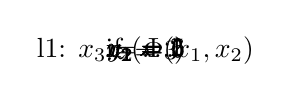
\begin{tikzpicture}
  \node (start) {};
  \node (a) {$x_1 = 5$};
  \node (b) {$x_2 = 6$};
  \node (c) {if ($\ldots$)};
  \node (d) {$y_1 = 1$};
  \node (e) {$y_2 = 2$};
  \node (f) {$z = 3$};
  \node (g) {l1: $x_3 = \Phi(x_1, x_2)$};
  \draw[->] (start) -- (a);
  \draw[->] (start) -- (b);
  \draw[->] (a) -- (g);
  \draw[->] (b) -- (c);
  \draw[->] (c) -- (d);
  \draw[->] (c) -- (e);
  \draw[->] (d) -- (f);
  \draw[->] (e) -- (f);
  \draw[->] (f) -- (g);
\end{tikzpicture}
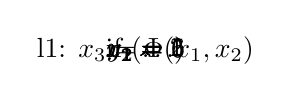
\begin{tikzpicture}
  \node (start) {};
  \node (a) {$x_1 = 5$};
  \node (b) {$x_2 = 6$};
  \node (c) {if ($\ldots$)};
  \node (d) {$y_1 = 1$};
  \node (e) {$y_2 = 2$};
  \node (g) {l1: $x_3 = \Phi(x_1, x_2)$};
  \draw[->] (start) -- (a);
  \draw[->] (start) -- (b);
  \draw[->] (a) -- (g);
  \draw[->] (b) -- (c);
  \draw[->] (c) -- (d);
  \draw[->] (c) -- (e);
  \draw[->] (d) -- (g);
  \draw[->] (e) -- (g);
\end{tikzpicture}
\caption{Optimising an SSA-form machine}
\label{fig:ssa_cfg1}
\end{figure}

\todo{Not actually sure how interesting this is, now that I've written it down.}

\subsection{Building write-side \StateMachines}

Once SLI has obtained the read-side \StateMachine, it can analyse it to determine which loads affect the ultimate prediction, and then compare this set to the dynamic model to determine which stores might potentially influence it.
The analysis must then consider all dynamic paths of $N^w$ instructions which contain at least one of those store operations.
As when building read-side \StateMachines, it would be possible to do this by enumerating all possible such paths and compiling each to an independent \StateMachine, but that would be extremely wasteful.
SLI uses a somewhat more intelligent approach.
The basic approach here is essentially the same as that used for read-side \StateMachines: convert the set of dynamic paths into a (hopefully much smaller) set of acyclic control-flow graphs and then compile those CFGs into \StateMachines.
The details of the algorithms used are, however, slightly different.

\subsubsection{Finding relevant stores}

The first phase of building the write-side \StateMachines is to determine which stores in the program might possibly be relevant.
These are the ones which might affect the result produced by the read-side \StateMachine.
Finding these is straightforward:

\begin{itemize}
\item
  Remove all of the optional annotations from the read-side \StateMachine.
  These are the side effects which provide additional information to the analysis but do not themselves affect the semantics of the \StateMachine, such as assert or stack-layout side effects.
\item
  Simplify the resulting machine down as far as possible.
  Removing annotations can sometimes enable further optimisations if, for instance, two path through the \StateMachine are identical except for inserting an additional intermediate function in the call stack and that intermediate function does not itself perform any relevant operations.
\item
  Find all of the memory load operations which remain the simplified machine.
\item
  Examine the model collected during the dynamic analysis phase to locate all of the stores which might access the same memory location as one of those loads.
  This effectively assumes both that the dynamic analysis phase has correctly captured the program's internal type system and that the program has a particular memory safety property.
  \todo{Say more.}
\end{itemize}

\subsubsection{Build write-side CFGs}
\todo{This has far more pages than it really deserves, although most
  of them are diagrams, so I guess it's not too bad.}

The input to this phase of the analysis is a set of potentially relevant static store instructions, and the analysis must build a collection of acyclic CFGs which cover all possible paths through the program which use at least one of those static instructions and which contain at most $N_w$ instructions.
\editorial{That's not quite the problem definition I used earlier, but it's a bit easier to describe.}

One important assumption here is that the set of potentially relevant store instructions is complete, in the sense that no instruction not in that set can influence the behaviour of the load machine (this follows from the assumption that the dynamic model is itself complete).
This implies that the only parts of the dynamic write path which are actually important are the potentially relevant store instructions; everything else simply acts to constrain the behaviour of those instructions.
That in turn means that it is safe to ignore any prefix or suffix of a dynamic path which does not involve any potentially-relevant store instructions, or, to put it another way, the store CFGs only need to represent dynamic paths which start and end with potentially-relevant instructions.
This is a useful simplification.

The algorithm begins by building a partial static CFG starting at each of the potentially-relevant store instructions and covering every instruction reachable within $N_w$ instructions of that point.
As with read-side CFGs, called functions are effectively inlined into each call site, and returns from the function containing the potentially-relevant store are handled by replacing the instruction with one with a synthesised call stack and restarting.
The CFGs generated by different starting instructions will often overlap; this is handled by sharing nodes between the relevant CFGs.
The resulting CFG is then trimmed to remove any instructions which cannot reach a potentially-relevant store within $N_w$ instructions.

At this point, the CFG represents a fragment of the program and contains every instruction which might be on one of the trimmed dynamic paths which need to be represented by the output CFG, and it only remains to remove any cycles from it.
As with read-side CFGs, this is accomplished by duplicating nodes so as to unroll loops until any path which uses the loop more than once must be longer than $N_w$ instructions and can hence be discarded.
There is, however, one important difference: in the read-side CFG, we are interested in any path which terminates at a specific point, whereas in the write-side CFG we need to preserve any path which starts and ends with any member of a set of interesting instructions.
This makes it more difficult to determine when a loop has been unrolled sufficiently, as it is no longer sufficient to just check the distance to a nominated target instruction.
SLI solves this problem by labelling each node in the graph with information about where it might occur in an interesting path.
This label consists of:

\begin{itemize}
\item
  For each possibly-relevant store, the minimum distance from that store to the labelled node.
\item
  For each possible-relevant store, the minimum distance from the labelled node to that store or any of its duplicates.
\end{itemize}

We only need to consider paths of length $N_w$ or less which start with one of the potentially-relevant stores and which end with a potentially-relevant store or one of its duplicates.
Therefore, if, for any node, the minimum of the first type of label plus the minimum of the second type of label exceeds $N_w$ the node can be safely discarded.
This allows us to break cycles once they have been unrolled far enough.

\begin{algorithmic}
  \STATE {Compute initial labelling of graph}
  \FORALL {$t$ in the set of potentially-relevant stores}
    \WHILE {graph rooted at $t$ is not cycle-free}
       \STATE $edge \gets findEdgeToBeBroken(t, \{\})$
       \STATE $newLabel \gets combineLabels(\text{current label of } edge.start, \text{current label of } edge.end)$
       \IF {$min(newLabel.minFrom) + min(newLabel.minTo) > N_w$}
           \STATE {remove $edge$}
       \ELSE
           \STATE $newNode <- \text{duplicate } edge.end$
           \FORALL {Edges $e$ leaving $edge.end$}
              \STATE {Create a new edge from $newNode$ to $e.end$}
           \ENDFOR
           \STATE {Set label of $newNode$ to $newLabel$}
           \STATE {Replace $edge$ with an edge from $edge.start$ to $newNode$}
       \ENDIF
    \ENDWHILE
  \ENDFOR
\end{algorithmic}

\begin{tikzpicture}
  \node (A) at (0,2) [TrueCfgInstr] {A};
  \node (B) [CfgInstr, below=of A] {B} edge [in=30,out=-30,loop] ();
  \node (C) [TrueCfgInstr, below=of B] {C};
  \draw[->] (A) -- (B);
  \draw[->] (B) -- (C);
  \draw[->] (C) to [bend left=90] (A) node (edge1) [right,midway] {~~~~~~~~};
  \begin{pgfonlayer}{bg}
    \node(box1) [fill=black!10,fit=(A) (B) (C) (edge1)] {};
  \end{pgfonlayer}
  \draw node [right=of box1] {
    \begin{tabular}{lcccc}
      labels & min to A & min from A & min to C & min from C\\
      A & 0 & 0 & 2 & 1\\
      B & 2 & 1 & 1 & 2\\
      C & 1 & 2 & 0 & 0\\
    \end{tabular}
  };
\end{tikzpicture}

\begin{tikzpicture}
  \node (A) at (0,2) [TrueCfgInstr] {A};
  \node (B) [CfgInstr, below=of A] {B};
  \node (B1) [NewCfgInstr, right=of B] {B1};
  \node (C) [TrueCfgInstr, below=of B] {C};
  \draw[->] (A) -- (B);
  \draw[->] (B) -- (C);
  \draw[->] (B) to [bend left=10] (B1);
  \draw[->,swungEdge] (B1) to [bend left=10] (B);
  \draw[->] (B1) -- (C);
  \draw[->] (C) to [bend left=90] (A) node (edge1) [right,midway] {~~~~~~~~};
  \begin{pgfonlayer}{bg}
    \node(box1) [fill=black!10,fit=(A) (B) (B1) (C) (edge1)] {};
  \end{pgfonlayer}
  \draw node [right=of box1] {
    \begin{tabular}{lcccc}
      labels & min to A & min from A & min to C & min from C\\
      A  & 0 & 0 & 2 & 1\\
      B  & 2 & 1 & 1 & 2\\
      C  & 1 & 2 & 0 & 0\\
      B1 & 2 & 2 & 1 & 3\\
    \end{tabular}
    (dupe B)
  };
\end{tikzpicture}

\begin{tikzpicture}
  \node (A) at (0,2) [TrueCfgInstr] {A};
  \node (B) [CfgInstr, below=of A] {B};
  \node (B1) [CfgInstr, right=of B] {B1};
  \node (C) [TrueCfgInstr, below=of B] {C};
  \node (A1) [NewCfgInstr,right=of C] {A1};
  \draw[->] (A) -- (B);
  \draw[->,swungEdge] (A1) -- (B);
  \draw[->] (B) -- (C);
  \draw[->] (B) to [bend left=10] (B1);
  \draw[->] (B1) -- (C);
  \draw[->] (B1) to [bend left=10] (B);
  \draw[->] (C) -- (A1);
  \begin{pgfonlayer}{bg}
    \node(box1) [fill=black!10,fit=(A) (B) (B1) (C) (edge1)] {};
  \end{pgfonlayer}
  \draw node [right=of box1] {
    \begin{tabular}{lcccc}
      labels & min to A & min from A & min to C & min from C\\
      A  & 0 & 0 & 2 & $\infty$\\
      A1 & 0 & 3 & 2 & 1\\
      B  & 2 & 1 & 1 & 2\\
      C  & 1 & 2 & 0 & 0\\
      B1 & 2 & 2 & 1 & 3\\
    \end{tabular}
    (dupe A)
  };
\end{tikzpicture}

\begin{tikzpicture}
  \node (A) at (0,2) [TrueCfgInstr] {A};
  \node (B) [CfgInstr, below=of A] {B};
  \node (B1) [CfgInstr, right=of B] {B1};
  \node (B2) [NewCfgInstr, right=of B1] {B2};
  \node (C) [TrueCfgInstr, below=of B] {C};
  \node (A1) [DupeCfgInstr,right=of C] {A1};
  \draw[->] (A) -- (B);
  \draw[->] (A1) -- (B);
  \draw[->] (B) -- (C);
  \draw[->] (B) -- (B1);
  \draw[->,swungEdge] (B1) to [bend left=10] (B2);
  \draw[->] (B1) -- (C);
  \draw[->] (B2) to [bend left=10] (B1);
  \draw[->] (B2) -- (C);
  \draw[->] (C) -- (A1);
  \begin{pgfonlayer}{bg}
    \node(box1) [fill=black!10,fit=(A) (A1) (B) (B1) (B2) (C) (edge1)] {};
  \end{pgfonlayer}
  \draw node [right=of box1] {
    \begin{tabular}{lcccc}
      labels & min to A & min from A & min to C & min from C\\
      A  & 0 & 0 & 2 & $\infty$\\
      A1 & 0 & 3 & 2 & 1\\
      B  & 2 & 1 & 1 & 2\\
      C  & 1 & 2 & 0 & 0\\
      B1 & 2 & 2 & 1 & 3\\
      B2 & 2 & 3 & 1 & 4\\
    \end{tabular}
  };
\end{tikzpicture}

\begin{tikzpicture}
  \node (A) at (0,2) [TrueCfgInstr] {A};
  \node (B) [CfgInstr, below=of A] {B};
  \node (B1) [CfgInstr, right=of B] {B1};
  \node (B2) [CfgInstr, right=of B1] {B2};
  \node (A1) [DupeCfgInstr,right=of C] {A1};
  \node (C) [TrueCfgInstr, below=of B] {C};
  \node (B3) [NewCfgInstr, below=of A1] {B3};
  \draw[->] (A) -- (B);
  \draw[->,swungEdge] (A1) -- (B3);
  \draw[->] (B) -- (C);
  \draw[->] (B) -- (B1);
  \draw[->] (B1) to [bend left=10] (B2);
  \draw[->] (B1) -- (C);
  \draw[->] (B2) to [bend left=10] (B1);
  \draw[->] (B2) -- (C);
  \draw[->] (B3) -- (C);
  \draw[->] (B3) to [bend right=45] (B1);
  \draw[->] (C) -- (A1);
  \begin{pgfonlayer}{bg}
    \node(box1) [fill=black!10,fit=(A) (A1) (B) (B1) (B2) (B3) (C) (edge1)] {};
  \end{pgfonlayer}
  \draw node [right=of box1] {
    \begin{tabular}{lcccc}
      labels & min to A & min from A & min to C & min from C\\
      A  & 0 & 0 & 2 & $\infty$\\
      A1 & 0 & 3 & 2 & 1\\
      B  & 2 & 1 & 1 & $\infty$\\
      C  & 1 & 2 & 0 & 0\\
      B1 & 2 & 2 & 1 & 3\\
      B2 & 2 & 3 & 1 & 4\\
      B3 & 2 & 4 & 1 & 2\\
    \end{tabular}
  };
\end{tikzpicture}

\begin{tikzpicture}
  \node (A) at (0,2) [TrueCfgInstr] {A};
  \node (B) [CfgInstr, below=of A] {B};
  \node (B1) [CfgInstr, right=of B] {B1};
  \node (B2) [CfgInstr, right=of B1] {B2};
  \node (A1) [DupeCfgInstr,right=of C] {A1};
  \node (C) [TrueCfgInstr, below=of B] {C};
  \node (B3) [CfgInstr, below=of A1] {B3};
  \draw[->] (A) -- (B);
  \draw[->] (A1) -- (B3);
  \draw[->] (B) -- (C);
  \draw[->] (B) -- (B1);
  \draw[->] (B1) to [bend left=10] (B2);
  \draw[->] (B1) -- (C);
  \draw[->] (B2) to [bend left=10] (B1);
  \draw[->,killEdge] (B2) to [bend left=10] (B1);
  \draw[->] (B2) -- (C);
  \draw[->] (B3) -- (C);
  \draw[->] (B3) to [bend right=45] (B1);
  \draw[->] (C) -- (A1);
  \begin{pgfonlayer}{bg}
    \node(box1) [fill=black!10,fit=(A) (A1) (B) (B1) (B2) (B3) (C) (edge1)] {};
  \end{pgfonlayer}
  \draw node [right=of box1] {
    \begin{tabular}{lcccc}
      labels & min to A & min from A & min to C & min from C\\
      A  & 0 & 0 & 2 & $\infty$\\
      A1 & 0 & 3 & 2 & 1\\
      B  & 2 & 1 & 1 & $\infty$\\
      C  & 1 & 2 & 0 & 0\\
      B1 & 2 & 2 & 1 & 3\\
      B2 & 2 & 3 & 1 & 4\\
      New label & 2 & 4 & 1 & 5\\
    \end{tabular}
  };
\end{tikzpicture}

\begin{tikzpicture}
  \node (A) at (0,2) [TrueCfgInstr] {A};
  \node (B) [CfgInstr, below=of A] {B};
  \node (B1) [CfgInstr, right=of B] {B1};
  \node (B2) [CfgInstr, right=of B1] {B2};
  \node (A1) [DupeCfgInstr,right=of C] {A1};
  \node (C) [TrueCfgInstr, below=of B] {C};
  \node (B3) [CfgInstr, below=of A1] {B3};
  \node (C1) [NewCfgInstr, below=of B3] {C1};
  \draw[->] (A) -- (B);
  \draw[->] (A1) -- (B3);
  \draw[->] (B) -- (C);
  \draw[->] (B) -- (B1);
  \draw[->] (B1) -- (B2);
  \draw[->] (B1) -- (C);
  \draw[->] (B2) -- (C);
  \draw[->] (B3) to [bend left=45] (B1);
  \draw[->] (C) -- (A1);
  \draw[->] (C1) to [bend right=90] (A1);
  \draw[->,swungEdge] (B3) -- (C1);
  \begin{pgfonlayer}{bg}
    \node(box1) [fill=black!10,fit=(A) (A1) (B) (B1) (B2) (B3) (C) (C1) (edge1)] {};
  \end{pgfonlayer}
  \draw node [right=of box1] {
    \begin{tabular}{lcccc}
      labels & min to A & min from A & min to C & min from C\\
      A  & 0 & 0 & 2 & $\infty$\\
      A1 & 0 & 3 & 2 & 1\\
      B  & 2 & 1 & 1 & $\infty$\\
      C  & 1 & 2 & 0 & 0\\
      B1 & 2 & 2 & 1 & 3\\
      B2 & 2 & 3 & 1 & 4\\
      C3 & 1 & 4 & 0 & 3\\
    \end{tabular}
  };
\end{tikzpicture}

\begin{tikzpicture}
  \node (A) at (0,2) [TrueCfgInstr] {A};
  \node (B) [CfgInstr, below=of A] {B};
  \node (B1) [CfgInstr, right=of B] {B1};
  \node (B2) [CfgInstr, right=of B1] {B2};
  \node (A1) [DupeCfgInstr,right=of C] {A1};
  \node (C) [TrueCfgInstr, below=of B] {C};
  \node (B3) [CfgInstr, below=of A1] {B3};
  \node (C1) [DupeCfgInstr, below=of B3] {C1};
  \node (B4) [NewCfgInstr, right=of B3] {B4};
  \draw[->] (A) -- (B);
  \draw[->] (A1) -- (B3);
  \draw[->] (B) -- (C);
  \draw[->] (B) -- (B1);
  \draw[->] (B1) -- (B2);
  \draw[->] (B1) -- (C);
  \draw[->] (B2) -- (C);
  \draw[->,swungEdge] (B3) -- (B4);
  \draw[->] (C) -- (A1);
  \draw[->] (C1) to [bend right=45] (A1);
  \draw[->] (B3) -- (C1);
  \draw[->] (B4) -- (C);
  \draw[->] (B4) -- (B2);
  \begin{pgfonlayer}{bg}
    \node(box1) [fill=black!10,fit=(A) (A1) (B) (B1) (B2) (B3) (C) (C1) (edge1)] {};
  \end{pgfonlayer}
  \draw node [right=of box1] {
    \begin{tabular}{lcccc}
      labels & min to A & min from A & min to C & min from C\\
      A  & 0 & 0 & 2 & $\infty$\\
      A1 & 0 & 3 & 2 & 1\\
      B  & 2 & 1 & 1 & $\infty$\\
      C  & 1 & 2 & 0 & 0\\
      B1 & 2 & 2 & 1 & $\infty$\\
      B2 & 2 & 3 & 1 & 4\\
      C3 & 1 & 4 & 0 & 3\\
      B4 & 2 & 5 & 1 & 3\\
    \end{tabular}
  };
\end{tikzpicture}

\begin{tikzpicture}
  \node (A) at (0,2) [TrueCfgInstr] {A};
  \node (B) [CfgInstr, below=of A] {B};
  \node (B1) [CfgInstr, right=of B] {B1};
  \node (B2) [CfgInstr, right=of B1] {B2};
  \node (A1) [DupeCfgInstr,right=of C] {A1};
  \node (C) [TrueCfgInstr, below=of B] {C};
  \node (B3) [CfgInstr, below=of A1] {B3};
  \node (C1) [DupeCfgInstr, below=of B3] {C1};
  \node (B4) [CfgInstr, right=of B3] {B4};
  \node (A2) [NewCfgInstr, left=of C1] {A2};
  \draw[->] (A) -- (B);
  \draw[->] (A1) -- (B3);
  \draw[->] (B) -- (C);
  \draw[->] (B) -- (B1);
  \draw[->] (B1) -- (B2);
  \draw[->] (B1) -- (C);
  \draw[->] (B2) -- (C);
  \draw[->] (B3) -- (B4);
  \draw[->] (C) -- (A1);
  \draw[->,swungEdge] (C1) -- (A2);
  \draw[->] (B3) -- (C1);
  \draw[->] (B4) -- (C);
  \draw[->] (B4) -- (B2);
  \draw[->] (A2) -- (B3);
  \begin{pgfonlayer}{bg}
    \node(box1) [fill=black!10,fit=(A) (A1) (A2) (B) (B1) (B2) (B3) (C) (C1) (edge1)] {};
  \end{pgfonlayer}
  \draw node [right=of box1] {
    \begin{tabular}{lcccc}
      labels & min to A & min from A & min to C & min from C\\
      A  & 0 & 0 & 2 & $\infty$\\
      A1 & 0 & 3 & 2 & 1\\
      B  & 2 & 1 & 1 & $\infty$\\
      C  & 1 & 2 & 0 & 0\\
      B1 & 2 & 2 & 1 & $\infty$\\
      B2 & 2 & 3 & 1 & 4\\
      C3 & 1 & 4 & 0 & 3\\
      B4 & 2 & 5 & 1 & 3\\
      A2 & 0 & 6 & 2 & 4\\
    \end{tabular}
  };
\end{tikzpicture}

\begin{tikzpicture}
  \node (A) at (0,2) [TrueCfgInstr] {A};
  \node (B) [CfgInstr, below=of A] {B};
  \node (B1) [CfgInstr, right=of B] {B1};
  \node (B2) [CfgInstr, right=of B1] {B2};
  \node (A1) [DupeCfgInstr,right=of C] {A1};
  \node (C) [TrueCfgInstr, below=of B] {C};
  \node (B3) [CfgInstr, below=of A1] {B3};
  \node (C1) [DupeCfgInstr, below=of B3] {C1};
  \node (B4) [CfgInstr, right=of B3] {B4};
  \node (A2) [DupeCfgInstr, left=of C1] {A2};
  \node (C2) [NewCfgInstr, below=of B4] {C2};
  \draw[->] (A) -- (B);
  \draw[->] (A1) -- (B3);
  \draw[->] (B) -- (C);
  \draw[->] (B) -- (B1);
  \draw[->] (B1) -- (B2);
  \draw[->] (B1) -- (C);
  \draw[->] (B2) -- (C);
  \draw[->] (B3) -- (B4);
  \draw[->] (C) -- (A1);
  \draw[->] (C1) -- (A2);
  \draw[->] (B3) -- (C1);
  \draw[->,swungEdge] (B4) -- (C2);
  \draw[->] (B4) -- (B2);
  \draw[->] (A2) -- (B3);
  \draw[->] (C2) -- (A1);
  \begin{pgfonlayer}{bg}
    \node(box1) [fill=black!10,fit=(A) (A1) (A2) (B) (B1) (B2) (B3) (C) (C1) (C2) (edge1)] {};
  \end{pgfonlayer}
  \draw node [right=of box1] {
    \begin{tabular}{lcccc}
      labels & min to A & min from A & min to C & min from C\\
      A  & 0 & 0 & 2 & $\infty$\\
      A1 & 0 & 3 & 2 & 1\\
      B  & 2 & 1 & 1 & $\infty$\\
      C  & 1 & 2 & 0 & 0\\
      B1 & 2 & 2 & 1 & $\infty$\\
      B2 & 2 & 3 & 1 & 4\\
      C3 & 1 & 4 & 0 & 3\\
      B4 & 2 & 5 & 1 & 3\\
      A2 & 0 & 6 & 2 & 4\\
      C2 & 1 & 6 & 0 & 4\\
    \end{tabular}
  };
\end{tikzpicture}

\begin{tikzpicture}
  \node (A) at (0,2) [TrueCfgInstr] {A};
  \node (B) [CfgInstr, below=of A] {B};
  \node (B1) [CfgInstr, right=of B] {B1};
  \node (B2) [CfgInstr, right=of B1] {B2};
  \node (A1) [DupeCfgInstr,right=of C] {A1};
  \node (C) [TrueCfgInstr, below=of B] {C};
  \node (B3) [CfgInstr, below=of A1] {B3};
  \node (C1) [DupeCfgInstr, below=of B3] {C1};
  \node (B4) [CfgInstr, right=of B3] {B4};
  \node (A2) [DupeCfgInstr, left=of C1] {A2};
  \node (C2) [DupeCfgInstr, below=of B4] {C2};
  \draw[->] (A) -- (B);
  \draw[->] (A1) -- (B3);
  \draw[->] (B) -- (C);
  \draw[->] (B) -- (B1);
  \draw[->] (B1) -- (B2);
  \draw[->] (B1) -- (C);
  \draw[->] (B2) -- (C);
  \draw[->] (B3) -- (B4);
  \draw[->] (C) -- (A1);
  \draw[->] (C1) -- (A2);
  \draw[->] (B3) -- (C1);
  \draw[->] (B4) -- (C2);
  \draw[->] (B4) -- (B2);
  \draw[->] (A2) -- (B3);
  \draw[->,killEdge] (A2) -- (B3);
  \draw[->] (C2) -- (A1);
  \begin{pgfonlayer}{bg}
    \node(box1) [fill=black!10,fit=(A) (A1) (A2) (B) (B1) (B2) (B3) (C) (C1) (C2) (edge1)] {};
  \end{pgfonlayer}
  \draw node [right=of box1] {
    \begin{tabular}{lcccc}
      labels & min to A & min from A & min to C & min from C\\
      A  & 0 & 0 & 2 & $\infty$\\
      A1 & 0 & 3 & 2 & 1\\
      B  & 2 & 1 & 1 & $\infty$\\
      C  & 1 & 2 & 0 & 0\\
      B1 & 2 & 2 & 1 & $\infty$\\
      B2 & 2 & 3 & 1 & 4\\
      C3 & 1 & 4 & 0 & 3\\
      B4 & 2 & 5 & 1 & 3\\
      A2 & 0 & 6 & 2 & 4\\
      C2 & 1 & 6 & 0 & 4\\
      New label & 2 & 7 & 1 & 5\\
    \end{tabular}\\
    (Dupe B5)
  };
\end{tikzpicture}

\begin{tikzpicture}
  \node (A) at (0,2) [TrueCfgInstr] {A};
  \node (B) [CfgInstr, below=of A] {B};
  \node (B1) [CfgInstr, right=of B] {B1};
  \node (B2) [CfgInstr, right=of B1] {B2};
  \node (A1) [DupeCfgInstr,right=of C] {A1};
  \node (C) [TrueCfgInstr, below=of B] {C};
  \node (B3) [CfgInstr, below=of A1] {B3};
  \node (C1) [DupeCfgInstr, below=of B3] {C1};
  \node (B4) [CfgInstr, right=of B3] {B4};
  \node (A2) [DupeCfgInstr, left=of C1] {A2};
  \node (C2) [DupeCfgInstr, below=of B4] {C2};
  \draw[->] (A) -- (B);
  \draw[->] (A1) -- (B3);
  \draw[->] (B) -- (C);
  \draw[->] (B) -- (B1);
  \draw[->] (B1) -- (B2);
  \draw[->] (B1) -- (C);
  \draw[->] (B2) -- (C);
  \draw[->] (B3) -- (B4);
  \draw[->] (C) -- (A1);
  \draw[->] (C1) -- (A2);
  \draw[->] (B3) -- (C1);
  \draw[->] (B4) -- (C2);
  \draw[->] (B4) -- (B2);
  \draw[->] (C2) -- (A1);
  \draw[->,killEdge] (C2) -- (A1);
  \begin{pgfonlayer}{bg}
    \node(box1) [fill=black!10,fit=(A) (A1) (A2) (B) (B1) (B2) (B3) (C) (C1) (C2) (edge1)] {};
  \end{pgfonlayer}
  \draw node [right=of box1] {
    \begin{tabular}{lcccc}
      labels & min to A & min from A & min to C & min from C\\
      A  & 0 & 0 & 2 & $\infty$\\
      A1 & 0 & 3 & 2 & 1\\
      B  & 2 & 1 & 1 & $\infty$\\
      C  & 1 & 2 & 0 & 0\\
      B1 & 2 & 2 & 1 & $\infty$\\
      B2 & 2 & 3 & 1 & 4\\
      C3 & 1 & 4 & 0 & 3\\
      B4 & 2 & 5 & 1 & 3\\
      A2 & 0 & 6 & 2 & 4\\
      C2 & 1 & 6 & 0 & 4\\
      New label & 0 & 7 & 2 & 5\\
    \end{tabular}\\
    (Dupe A1)
  };
\end{tikzpicture}

\begin{tikzpicture}
  \node (A) at (0,2) [TrueCfgInstr] {A};
  \node (B) [CfgInstr, below=of A] {B};
  \node (B1) [CfgInstr, right=of B] {B1};
  \node (B2) [CfgInstr, right=of B1] {B2};
  \node (A1) [DupeCfgInstr,right=of C] {A1};
  \node (C) [TrueCfgInstr, below=of B] {C};
  \node (B3) [CfgInstr, below=of A1] {B3};
  \node (C1) [DupeCfgInstr, below=of B3] {C1};
  \node (B4) [CfgInstr, right=of B3] {B4};
  \node (A2) [DupeCfgInstr, left=of C1] {A2};
  \node (C2) [DupeCfgInstr, below=of B4] {C2};
  \node (C3) [NewCfgInstr, right=of A1] {C3};
  \draw[->] (A) -- (B);
  \draw[->] (A1) -- (B3);
  \draw[->] (B) -- (C);
  \draw[->] (B) -- (B1);
  \draw[->] (B1) -- (B2);
  \draw[->] (B1) -- (C);
  \draw[->,swungEdge] (B2) -- (C3);
  \draw[->] (B3) -- (B4);
  \draw[->] (C) -- (A1);
  \draw[->] (C1) -- (A2);
  \draw[->] (B3) -- (C1);
  \draw[->] (B4) -- (C2);
  \draw[->] (B4) to [bend left=45] (B2);
  \draw[->] (C3) -- (A1);
  \begin{pgfonlayer}{bg}
    \node(box1) [fill=black!10,fit=(A) (A1) (A2) (B) (B1) (B2) (B3) (C) (C1) (C2) (C3) (edge1)] {};
  \end{pgfonlayer}
  \draw node [right=of box1] {
    \begin{tabular}{lcccc}
      labels & min to A & min from A & min to C & min from C\\
      A  & 0 & 0 & 2 & $\infty$\\
      A1 & 0 & 3 & 2 & 1\\
      B  & 2 & 1 & 1 & $\infty$\\
      C  & 1 & 2 & 0 & 0\\
      B1 & 2 & 2 & 1 & $\infty$\\
      B2 & 2 & 3 & 1 & 4\\
      C3 & 1 & 4 & 0 & 3\\
      B4 & 2 & 5 & 1 & 3\\
      A2 & 0 & 6 & 2 & 4\\
      C2 & 1 & 6 & 0 & 4\\
      C3 & 1 & 4 & 0 & 5\\
    \end{tabular}
  };
\end{tikzpicture}

\begin{tikzpicture}
  \node (A) at (0,2) [TrueCfgInstr] {A};
  \node (B) [CfgInstr, below=of A] {B};
  \node (B1) [CfgInstr, right=of B] {B1};
  \node (B2) [CfgInstr, right=of B1] {B2};
  \node (A1) [DupeCfgInstr,right=of C] {A1};
  \node (C) [TrueCfgInstr, below=of B] {C};
  \node (B3) [CfgInstr, below=of A1] {B3};
  \node (C1) [DupeCfgInstr, below=of B3] {C1};
  \node (B4) [CfgInstr, right=of B3] {B4};
  \node (A2) [DupeCfgInstr, left=of C1] {A2};
  \node (C2) [DupeCfgInstr, below=of B4] {C2};
  \node (C3) [DupeCfgInstr, right=of A1] {C3};
  \draw[->] (A) -- (B);
  \draw[->] (A1) -- (B3);
  \draw[->] (B) -- (C);
  \draw[->] (B) -- (B1);
  \draw[->] (B1) -- (B2);
  \draw[->] (B1) -- (C);
  \draw[->] (B2) -- (C3);
  \draw[->] (B3) -- (B4);
  \draw[->] (C) -- (A1);
  \draw[->] (C1) -- (A2);
  \draw[->] (B3) -- (C1);
  \draw[->] (B4) -- (C2);
  \draw[->] (B4) to [bend left=45] (B2);
  \draw[->,killEdge] (B4) to [bend left=45] (B2);
  \draw[->] (C3) -- (A1);
  \begin{pgfonlayer}{bg}
    \node(box1) [fill=black!10,fit=(A) (A1) (A2) (B) (B1) (B2) (B3) (C) (C1) (C2) (C3) (edge1)] {};
  \end{pgfonlayer}
  \draw node [right=of box1] {
    \begin{tabular}{lcccc}
      labels & min to A & min from A & min to C & min from C\\
      A  & 0 & 0 & 2 & $\infty$\\
      A1 & 0 & 3 & 2 & 1\\
      B  & 2 & 1 & 1 & $\infty$\\
      C  & 1 & 2 & 0 & 0\\
      B1 & 2 & 2 & 1 & $\infty$\\
      B2 & 2 & 3 & 1 & $\infty$\\
      C3 & 1 & 4 & 0 & $\infty$\\
      B4 & 2 & 5 & 1 & 3\\
      A2 & 0 & 6 & 2 & 4\\
      C2 & 1 & 6 & 0 & 4\\
      C3 & 1 & 4 & 0 & 5\\
      New label & 2 & 6 & 1 & 4\\
    \end{tabular}
  };
\end{tikzpicture}

\begin{tikzpicture}
  \node (A) at (0,2) [TrueCfgInstr] {A};
  \node (B) [CfgInstr, below=of A] {B};
  \node (B1) [CfgInstr, right=of B] {B1};
  \node (B2) [CfgInstr, right=of B1] {B2};
  \node (A1) [DupeCfgInstr,right=of C] {A1};
  \node (C) [TrueCfgInstr, below=of B] {C};
  \node (B3) [CfgInstr, below=of A1] {B3};
  \node (C1) [DupeCfgInstr, below=of B3] {C1};
  \node (B4) [CfgInstr, right=of B3] {B4};
  \node (A2) [DupeCfgInstr, left=of C1] {A2};
  \node (C2) [DupeCfgInstr, below=of B4] {C2};
  \node (C3) [DupeCfgInstr, right=of A1] {C3};
  \draw[->] (A) -- (B);
  \draw[->] (A1) -- (B3);
  \draw[->] (B) -- (C);
  \draw[->] (B) -- (B1);
  \draw[->] (B1) -- (B2);
  \draw[->] (B1) -- (C);
  \draw[->] (B2) -- (C3);
  \draw[->] (B3) -- (B4);
  \draw[->] (C) -- (A1);
  \draw[->] (C1) -- (A2);
  \draw[->] (B3) -- (C1);
  \draw[->] (B4) -- (C2);
  \draw[->] (C3) -- (A1);
  \draw[->,killEdge] (C3) -- (A1);
  \begin{pgfonlayer}{bg}
    \node(box1) [fill=black!10,fit=(A) (A1) (A2) (B) (B1) (B2) (B3) (C) (C1) (C2) (C3) (edge1)] {};
  \end{pgfonlayer}
  \draw node [right=of box1] {
    \begin{tabular}{lcccc}
      labels & min to A & min from A & min to C & min from C\\
      A  & 0 & 0 & 2 & $\infty$\\
      A1 & 0 & 3 & 2 & 1\\
      B  & 2 & 1 & 1 & $\infty$\\
      C  & 1 & 2 & 0 & 0\\
      B1 & 2 & 2 & 1 & $\infty$\\
      B2 & 2 & 3 & 1 & $\infty$\\
      C3 & 1 & 4 & 0 & $\infty$\\
      B4 & 2 & 5 & 1 & 3\\
      A2 & 0 & 6 & 2 & 4\\
      C2 & 1 & 6 & 0 & 4\\
      C3 & 1 & 4 & 0 & 5\\
      New label & 0 & 5 & 2 & 6\\
    \end{tabular}
  };
\end{tikzpicture}

\begin{tikzpicture}
  \node (A) at (0,2) [TrueCfgInstr] {A};
  \node (B) [CfgInstr, below=of A] {B};
  \node (B1) [CfgInstr, right=of B] {B1};
  \node (B2) [CfgInstr, right=of B1] {B2};
  \node (A1) [DupeCfgInstr,right=of C] {A1};
  \node (C) [TrueCfgInstr, below=of B] {C};
  \node (B3) [CfgInstr, below=of A1] {B3};
  \node (C1) [DupeCfgInstr, below=of B3] {C1};
  \node (B4) [CfgInstr, right=of B3] {B4};
  \node (A2) [DupeCfgInstr, left=of C1] {A2};
  \node (C2) [DupeCfgInstr, below=of B4] {C2};
  \node (C3) [DupeCfgInstr, right=of A1] {C3};
  \draw[->] (A) -- (B);
  \draw[->] (A1) -- (B3);
  \draw[->] (B) -- (C);
  \draw[->] (B) -- (B1);
  \draw[->] (B1) -- (B2);
  \draw[->] (B1) -- (C);
  \draw[->] (B2) -- (C3);
  \draw[->] (B3) -- (B4);
  \draw[->] (C) -- (A1);
  \draw[->] (C1) -- (A2);
  \draw[->] (B3) -- (C1);
  \draw[->] (B4) -- (C2);
  \begin{pgfonlayer}{bg}
    \node(box1) [fill=black!10,fit=(A) (A1) (A2) (B) (B1) (B2) (B3) (C) (C1) (C2) (C3) (edge1)] {};
  \end{pgfonlayer}
  \draw node [right=of box1] {
    \begin{tabular}{lcccc}
      labels & min to A & min from A & min to C & min from C\\
      A  & 0 & 0 & 2 & $\infty$\\
      A1 & 0 & 3 & 2 & 1\\
      B  & 2 & 1 & 1 & $\infty$\\
      C  & 1 & 2 & 0 & 0\\
      B1 & 2 & 2 & 1 & $\infty$\\
      B2 & 2 & 3 & 1 & $\infty$\\
      C3 & 1 & 4 & 0 & $\infty$\\
      B4 & 2 & 5 & 1 & 3\\
      A2 & 0 & 6 & 2 & 4\\
      C2 & 1 & 6 & 0 & 4\\
      C3 & 1 & 4 & 0 & 5\\
    \end{tabular}
  };
\end{tikzpicture}


\subsection{Converting pairs of \StateMachines into verification conditions}

We now convert the pair of \StateMachines into a form of verification condition; that is, a predicate on the program's state which is satisfiable when the program contains a bug of the type being investigated\editorial{That isn't quite the usual definition of a verification condition.}.
SLI's completeness property is that if every possible \StateMachine pair which could be generated by the above algorithm is generated and each one is successfully converted to a verification condition (i.e. no part of the analysis times out), and none of the verification conditions are satisfiable, and the dynamic analysis is complete, the program will not contain any bugs of the class being investigated.

At a high level, the verification conditions are produced by considering each of the clauses of the bug definition in section~\todo{...} in turn, converting each into a \StateMachine, and then using symbolic execution to build a predicate saying when that clause might be satisfied.
These clause-conditions are then combined to produce the final verification condition for the original \StateMachine pair.

The rules for building each clause-condition are as follows:

\begin{itemize}
\item P valid -- \editorial{not sure what I'm going to say here -- P doesn't really exist at this stage, so this clause doesn't really make sense here.}
\item R valid -- true by construction of read machine, so the clause condition is just $1$.
\item W valid -- true by construction of write machine, so the clause condition is just $1$.
\item
  R atomic -- this rule states that the read \StateMachine must predict survival when run atomically.
  The \StateMachine to symbolically execute is then just the read-side \StateMachine, and the clause constraint is the rule which the symbolic executor derives for when the \StateMachine will survive.
\item
  W atomic -- this rule states that running the read \StateMachine after the write one must also predict survival.
  For this clause, we symbolically execute the concatenation of the two \StateMachines, and again the clause constraint is the rule when the \StateMachine will survive.
\item
  Crash possible -- this rule states that running the read and write \StateMachines in parallel must sometimes predict a crash.
  For this clause, we symbolically execute the cross-product parallel composition of the two \StateMachines.
  This time, the clause constraint is the rule for when the \StateMachine will crash.
\item
  W isolation -- used extensively when deriving write machine, to the extent that there's rarely any additional useful information to extract by this stage in the pipeline.
\item
  Concurrent -- model of program isn't strong enough to say anything useful about it.
\end{itemize}

We therefore produce three clause constraints for each \StateMachine pair, and must report a bug if they are simultaneously satisfiable.
As a minor optimisation, SLI assumes the R atomic clause is true when deriving the W atomic and crash clauses, and assumes that the W atomic clause is true when deriving the crash possible clause.

\subsubsection{Symbolically executing machines}

SLI uses a simple symbolic execution engine to evaluate machines and
determine when \StateMachines will crash.  The details of this are
fairly standard, and I only give a brief overview
here\editorial{\emph{Should} only give a brief overview; this ended up
  much more detailed than I'd expected.}.  The core data structure
used by the execution engine is a queue of (mostly) symbolic
configurations which the \StateMachine might occupy, and the main
operation is to take a state out of this queue, determine what the
\StateMachine might do next, and possibly add some additional
configurations to the queue to explore further.  Each configuration
contains:

\begin{itemize}
\item
  A mapping from temporary variable identifiers to the (symbolic) values of those variables.
\item
  A reference to the {\StateMachine}'s current (non-symbolic) state.
\item
  The order in which those temporaries were assigned to.
  As discussed in \S~\ref{sect:ssa}, SLI uses a slightly unusual form of single static assignment in which $\Phi$ nodes select their input variable based on which was assigned to most recently, rather than based on the preceding control flow, and this keeping track of that ordering allows that semantics to be implemented simply.
\item
  A log of all of the memory stores issued by the \StateMachine so far.
\item
  The current assumption.
  This is simply the conjunction of all of the conditions which are known to be true at this point in the execution.
\item
  The current ``path'' assumption.
  This is the subset of the current assumption which was introduced during the machine's execution.
  In other words, it is all of the things which are known to be true at this point in the execution but which were not known to be true at the start of the execution.
  This is often useful when building verification conditions, as discussed below.

  An alternative design would instead keep the path assumption and the initial assumption completely separate, and get rid of the current assumption, but this is slightly more convenient\editorial{think harder.}.
\end{itemize}\editorial{Plus some debug crap, but we don't care about that here.}

There are three possible outcomes from an execution: crash, survive, or escape.
The first two are obvious.
An escaping result indicates that the \StateMachine behaved in a way which indicates that this execution is not one of the ones which are of interest to the current bug.
This might, for instance, be because an assertion fails, or because a memory access (other than the one being investigated) dereferenced bad memory.
The exact treatment of escaping executions depends on how the results of the symbolic execution are to be used.

Implementing the various types of \StateMachine operation is straightforward:

\begin{itemize}
\item[cond]
  Check whether the assumption allows the condition to be simplified to a constant.
  If it does, simplify advance to the appropriate successor state.
  Otherwise, create two new successor configurations, moving one to the state's condition-true successor state and the other to the condition-false one and adding either the constraint (for the condition-true successor) or its inverse (for the condition-false one) to the current assumption and the path assumption.
\item[assert]
  Check whether the assumption allows the asserted value to be reduced to a constant.
  If it can, and that constant is one, simply move to the assertion's successor state.
  If the constant is zero, the execution escapes.
  Otherwise, if the asserted expression cannot be reduced to a constant, it is added to the current assumption and path assumption and the execution moves to the successor state.
\item[copy]
  Simplify the right-hand side of the copy as far as possible using the current assumption and then copy it to the appropriate place in the temporary variable table.
  The current assumption is then rewritten to replace any instances of the left-hand side of the copy with the simplified version of the right-hand side.
  The path assumption is not rewritten, and neither are the values of any of the other temporary values.
  \todo{I'm at least half convinced that this doesn't actually matter any more, due to changes elsewhere in the analysis pipeline.  Need to check that.}
\item[store]
  Assert that the pointer stored to is itself valid and then add the store to the log of issued stores.
\item[load]
  Assert that the pointer to be loaded is itself valid.
  Look through the log of issued stores, checking each one to see whether it might be storing to the location loaded by the load.
  If the load is unambiguously satisfied by a single store then create a single successor configuration then copy the value stored into the temporary variable targeted by the load using the same mechanism as used for copy side-effects.
  Otherwise, create one for each possible store, and potentially also one in which the load returns the initial value of memory.
\item[phi]
  Essentially as far copy operations.
\item
  Every operation is a no-op in the interpreter and simply moves to the next state.
  In particular, the execution engine ignores operations such as ``StartLayout'' and ``PointerAliasing'' which simply provide additional hints to the various \StateMachine simplification phases.
\end{itemize}

\todo{Possibly important that this uses the simplifier rather than the sat checker to see whether things reduce to a constant.}

Asserting that pointers are valid before performing memory operations is perhaps slightly surprising, as it means that the execution engine will never consider paths which crash due to dereferencing bad pointers.
This may appear odd in a system designed to investigate crashes due to dereferencing bad pointers.
However, it simply reflects the fact that, at this stage, SLI is only interested in a single possibly-crashing instruction, and so crashes at memory accesses prior to that one need to be ignored; asserting that dereferenced pointers are valid achieves that.
The interesting instruction itself is encoded without an explicit memory-accessing state (see \S~\todo{...}), so crashes there will not be affected by these assertions.

\todo{At one point, the execution engine was the reason we needed dynamic single assignment form.  I can't really see why it depends on it now, though, so that might be worth looking at more.}

\subsubsection{R atomic}

This rule states that the read machine must run to completion without crashing if run in isolation.
Once the read machine has been completely determined, this is in effect a condition on the states of the program which have to be considered: if the read machine would crash when run atomically in state S, any concurrency-related bugs detected starting from state S are highly unlikely to be interesting.
The first phase of building the verification condition is to build the condition.
To do so, the analysis first simplifies the probe machine on the assumption that it is running atomically and then symbolically executes it.
The constraint is then the conjunction of the inverses of the path conditions to reach crashing states.
Escaping executions are treated as crashing ones at this stage, so that they will not be considered by later stages of the analysis.

Path explosion: once you're assuming that the machine is completely atomic the state machine simplifier turns most machines into a simple predicate on the initial state and so the symbolic execution is pretty much trivial and there aren't really any paths to explode.
The main exception is where Phi nodes prevent us from simplifying control flow as far as we'd like.
Aliasing can also be an issue, but much less often than you'd expect.

\subsection{W atomic}

This rule requires that the read machine does not crash if run after the write machine has completed.
This, again, is about restricting the analysis to only consider bugs which are due to concurrency, and not any crashes which might be caused by other bugs.
For this rule, the analysis first concatenates the two machines by replacing the terminal states of the write machine with the first state in the read machine.
The resulting machine is then simplified and interpreted.
In this case, the symbolic execution engine is allowed to assume that the R atomic condition holds while performing this interpretation
The resulting path conditions are converted into a validity predicate in essentially the same way as they are for the R atomic rule.

Path explosion: again modest at this stage.
Most store machines just consist of a small number of store instructions (usually one, almost never more than three) and no control flow, and so we're effectively repeating the R atomic calculations in a slightly different initial state.
The aliasing problems are more complicated here but generally still not intractable.

\subsection{Crash possible}

This rule requires that the read machine must sometimes crash if run in parallel with the store machine.
To build this predicate, the analysis builds a new \StateMachine which is the cross product of the input read and write machines and then interprets that.
For this interpretation, escaping states, where assertions fail, are assumed to survive.
The final result is the disjunction of all of the path conditions which reach crashing states; combined with the validity condition, this describes all of the states which might exhibit a bug of the target class.

Complication: we arrange to build the machines in a way which avoids running either machine to completion in isolation.

I'm going to have to describe the algorithm here, because it's a little bit subtle.

Interesting properties of the algorithm:

\begin{itemize}
\item
  Needs to maintain atomic blocks.
\item
  Need to avoid considering the cases where either machine runs to completion before the other one starts.
\item
  Avoid considering both orderings of a load-store pair if they can't ever possibly access the same memory location.
  Slight complication: need to look past the current memory access to see if there's anything after it which might possibly race in an interesting way.
\item
  When you do need to consider both orderings, one of the orderings asserts that the two accesses access the same location and the other one doesn't.
\end{itemize}

Path explosion: much more of a concern now.
The cross machine will only have $O(n.m)$ states, which isn't \emph{too} bad, but once you combine that with the potential exponential blow-up in the execution engine proper's alias analysis it gets really quite messy.
You save a little because the validity predicate eliminates a bunch of possible configurations, though.

\subsection{Use of the induction rule}

The analysis uses a form of induction to eliminate some bugs.
The idea is that when analysing target instruction T, we can assume that there are no bugs of the target class for any other instruction T', and hence that the verification condition for T' is false.
Therefore, once we've finished generating the verification condition for a \StateMachine pair (L,S) we look at ``truncations'' of $L$, produced by cutting it off at each intermediate memory access, and generate verification conditions for each of them.
We can safely assume that these conditions are false while checking for satisfiability of the verification condition for the original \StateMachine pair.
This relies on the monotonicity property of the definition of crashes discussed in \S~\ref{sect:monotonicity}.

If this eliminates a crash then we log the fact that we've used induction, and then once every instruction has been completed we go back and check for cycles in this induction graph.
Usually, there aren't any, and so the induction is sound.
Otherwise, we count each such cycle as a single bug.

\todo{This isn't particularly effective, and it is very computationally expensive.}

\todo{Haven't actually found any cycles in that graph yet...}

\subsection{Completeness}
This is going to have a lot of forward references, because so many of the potential sources of uncompleteness are in the simplification bits, which I describe much later.

\subsection{Canonicalising machines}

The crash summaries generated by this analysis often contain a lot of redundant information, and this complicates later analysis, and also makes manually reviewing the generated summaries quite difficult.
SLI therefore implements some canonicalisation passes which remove some of this redundancy.

\todo{Caution, brain dump ahead}

\subsection{Phase 1 canonicalisation}
\subsubsection{Aliasing canonicalisation}
The aliasing table is converted into a predicate on the addresses accessed by the various memory accessing instructions and then added to the verification condition.

\subsubsection{Splitting SSA variables}
Two generations of a single SSA variable can be treated as independent variables provided that they're never used in the same $\Phi$ node.
This has no directly useful effects on any of the analyses which we perform, but it makes it a bit easier to canonicalise things.
In effect, this converts the machine part-way back out of SSA form.

\subsubsection{Thread ID canonicalisation}
\todo{Not worth mentioning}
The IDs of threads have no meaning beyond a simple equality test.
Therefore, if a single summary involves threads 1 and 3, but not thread 2, thread 3 could be renamed to thread 2 without it having any semantic effects.
Assigning thread IDs deterministically to members of the crash summary increases canonical-ness.

\subsubsection{Register canonicalisation}
Likewise, register identifiers are pretty much arbitrary, and differences which can be expressed by simple alpha conversion are generally not very interesting.
We therefore rename them in a way which is deterministic given the structure of the summary.
\todo{Analogy with De Bruijn indices?}

\subsubsection{CFG canonicalisation}
\todo{Should really do this, but don't.}

\subsection{Phase 2 canonicalisation}
The \StateMachines generated by the analysis can include some information which is helpful to the analysis but not usually directly relevant to understanding the bug which is being described.
The main examples are start and end of function markers and assertions.
For instance, suppose that the program looks like this:

\begin{verbatim}
f1() {
    if (complicated_condition1)
        return;
    g()
}
f2() {
    if (complicated_condition2)
        return;
    g()
}
\end{verbatim}

And that the \StateMachine for \verb|g| is \verb|g'|.
The state machines for $f1$ and $f2$ might then be:

\begin{verbatim}
f1: Assert (!complicated_condition1)
    g'
f2: Assert (!complicated_condition2)
    g'
\end{verbatim}

It is useful to retain \verb|complicated_condition1| and \verb|complicated_condition2| while generating the summaries, because they may contain information important to the bug, but once the summaries have been generated they become much less useful.
At this point, the only effect of the assertions is to make summaries which would otherwise be identical look like they are different.
Assertions are therefore removed completely during summary canonicalisation.

Likewise, function start and end markers are only used to determine when on-stack variables become live and dead, which is useful during analysis but becomes redundant once the full aliasing table is available.
They are therefore removed at this stage.

\subsection{Phase 3 canonicalisation}

Something about load canonicalisation, and why it has to be reversed later?

Important thing to worry about here is satisfiability of verification condition.

\subsubsection{Equality substitution}
Find equality constraints in the verification condition and use them to eliminate register from the summary.
This is done even when the result is more ``complex'' than the original input summary.
Approach is to find all of the registers which we can eliminate, then pick the one which occurs most often and eliminate it, then repeat until we can't eliminate anything else.

\todo{Need to come up with a coherent explanation of why doing this during analysis is bad.  Experimentally, it is, but it's not entirely obvious why that should be so.}

\subsubsection{Assume that the machines survive when run in isolation}
The verification condition includes the R atomic and W atomic assumptions.
These are necessary for the analysis to be valid, but tend not to provide a great deal of useful information.
This canonicalisation phase removes those components of the condition.
It re-derives the R atomic and W atomic assumptions as conditions, and then simplifies the verification condition and the \StateMachines under the assumption that they hold.

\subsubsection{Removal of redundant clauses}
The verification condition can sometimes include constraints on registers and memory locations which do not occur anywhere in any of the \StateMachines, usually because the \StateMachines have been simplified after the relevant part of the condition was derived.
In the simplest case, these variables are completely independent of the interesting variables.
\todo{Interesting variables are those which appear, or might appear (e.g. LD aliasing), in the \StateMachines.}
To find these, convert the verification condition to conjunctive normal form and then draw a graph whose nodes are variables and which has an edge between A and B if there is any clause in the verification condition which mentions both A and B.
Now find the connected components in this graph, $C_i$.
The verification condition can then be written as $f_1(C_1) \wedge f_2(C_2) \ldots$.
If any of the $C_i$ don't mention any variables in the interesting set then $f_i(C_i)$ can be set to true and hence discarded.

This is safe if $f_i(C_i)$ is satisfiable, which is the common case anyway.

\subsubsection{Removal of underspecified clauses}

If a free variable (i.e. one which isn't mentioned in the \StateMachines) occurs in precisely one place in the verification condition then it is referred to as being underspecified.
This means that, from the point of view of satisfiability checking, it can be set to anything at all, without reference to the rest of verification condition, which in turn means that certain clauses can become trivially satisfiable.
For instance, if $x$ is underspecified in this sense, and the verification condition includes the clause $x == y$, then a satisfiability checker would be able to select an $x$ to make that either true or false, and so our simplifications can assume that $x == y$ is either true or false according to whatever happens to be most convenient in context.

\subsubsection{Functionalisation/conditional independence}

This is analogous to the SSA transformation, but for boolean expressions rather than for programs.
The idea is that if you have a function of two free variables $f(x, y)$, you can treat $y$ as a function of $x$ to get $f(x, y_x)$
If $x$ and $y$ are boolean variables then you can then do a case split on $x$ to get $(x \wedge f(T, y_T)) \vee (\not{}x \wedge f(F, y_F))$.
$y_F$ and $y_T$ are then separate variables, and the two $f$ cases can be subjected to redundant clause removal and underspecified clause removal independently.

\todo{This is in dire need of an example.}

\todo{This is a lot like re-encoding the program's control flow into the verification condition, but in a way which is kind-of minimal and only contains the bits of control flow which are actually relevant.}

\subsection{Phase 4 canonicalisation}
The compound functions stuff.
Essentially, this notices if you have a lot of places in the verification condition/\StateMachine where you go $f(x, 5, 7)$, where $f$ is complex and only $x$ changes, and invents a new function to represent $f(..., 5, 7)$ and does a kind of backwards $\eta$ conversion to get rid of them.

\section{Building crash enforcement plans}

The previous phase of the algorithm produces a set of crash summaries, each of which consists of a read \StateMachine, a write \StateMachine, a verification condition, and an unrolled fragment of the program's control-flow graph.
Each summary is considered in turn and converted into a crash enforcement plan which, when applied to the program, will make the relevant bug more likely to reproduce.
We now illustrate the basic approach with a simple example before giving details of the algorithms used.

Suppose that the bug to be exhibited involves two threads:

\begin{verbatim}
int *global_ptr[];
void thread1(int idx1) {
    if (global_ptr[idx1])
        *global_ptr[idx1] = 7;
} 
void thread2(int idx2) {
    global_ptr[idx2] = NULL;
}
\end{verbatim}

Suppose further that these functions compile to this machine code:

\begin{verbatim}
thread1:

l1:   ADD global_ptr + idx1 -> reg1
l2:   LOAD *reg1 -> reg2
l3:   CMP 0, reg2
l4:   jmp_if_eq l7
l5:   LOAD *reg1 -> reg3
l6:   STORE 7 -> *reg3
l7:

thread2:

l8:   ADD global_ptr + idx2 -> reg4
l9:   STORE 0 -> *reg4
\end{verbatim}

There is a risk here that \verb|thread1| might crash if \verb|l9| is interleaved between \verb|l2| and \verb|l5| and \verb|idx1 == idx2|.
The previous analysis phase will produce \StateMachines something like these:

\begin{tikzpicture}
  \node[stateSideEffect,initial] (l2) {l2: Load $global\_ptr + idx1$ to $tmp1$};
  \node[stateIf,below = of l2] (l4) {l4: If $tmp1 == 0$?};
  \node[stateSideEffect, below = of l4] (l5) {l5: Load $global\_ptr + idx1$ to $tmp2$};
  \node[stateIf,below = of l5] (l6) {If $BadPtr(tmp2)$?};
  \node[stateTerminal,below right = of l6] (crash) {Crash};
  \node[stateTerminal,below left = of l6] (survive) {Survive};
  \draw[->] (l2) -- (l4);
  \draw[->] (l4) -- node {false} (l5);
  \draw[->] (l5) -- (l6);
  \draw[->] (l4.west) to [bend right=80] node {true} (survive);
  \draw[->] (l6.east) to [bend left=70] node {true} (crash);
  \draw[->] (l6.west) to [bend right=75] node {false} (survive);
  \begin{pgfonlayer}{bg}
    \node(box99) [fill=black!10,fit=(l2) (l4) (l5) (l6) (survive) (crash)] {};
  \end{pgfonlayer}

  \begin{scope} [xshift=8cm,yshift=-3cm]
    \node[stateSideEffect,initial] (l9) {l9: Store $0$ to $global\_ptr + idx2$};
    \node[stateTerminal,below=of l9] (end) {Finish};
    \draw[->] (l9) -- (end);
    \begin{pgfonlayer} {bg}
      \node [fill=black!10,fit=(l9) (end)] {};
    \end{pgfonlayer}
  \end{scope}
\end{tikzpicture}

With a verification condition that $idx1 == idx2$\editorial{Why does the verification condition not include the HB edges already?}.
Using symbolic execution it is then easy to show that, for the crash to happen, \verb|l9| must happen in between \verb|l2| and \verb|l5|, and so we can augment the \StateMachines with happens before edges as shown:

\begin{tikzpicture}
  \node[stateSideEffect,initial] (l2) {l2: Load $global\_ptr + idx1$ to $tmp1$};
  \node[stateIf,below = of l2] (l4) {l4: If $tmp1 == 0$?};
  \node[stateSideEffect, below = of l4] (l5) {l5: Load $global\_ptr + idx1$ to $tmp2$};
  \node[stateIf,below = of l5] (l6) {If $BadPtr(tmp2)$?};
  \node[stateTerminal,below right = of l6] (crash) {Crash};
  \node[stateTerminal,below left = of l6] (survive) {Survive};
  \draw[->] (l2) -- (l4);
  \draw[->] (l4) -- node {false} (l5);
  \draw[->] (l5) -- (l6);
  \draw[->] (l4.west) to [bend right=80] node {true} (survive);
  \draw[->] (l6.east) to [bend left=70] node {true} (crash);
  \draw[->] (l6.west) to [bend right=75] node {false} (survive);
  \begin{pgfonlayer}{bg}
    \node(box99) [fill=black!10,fit=(l2) (l4) (l5) (l6) (survive) (crash)] {};
  \end{pgfonlayer}

  \begin{scope} [xshift=8cm,yshift=-3cm]
    \node[stateSideEffect,initial] (l9) {l9: Store $0$ to $global\_ptr + idx2$};
    \node[stateTerminal,below=of l9] (end) {Finish};
    \draw[->] (l9) -- (end);
    \begin{pgfonlayer} {bg}
      \node [fill=black!10,fit=(l9) (end)] {};
    \end{pgfonlayer}
  \end{scope}

  \draw[->,happensBeforeEdge] (l2.south) -- (l9.north);
  \draw[->,happensBeforeEdge] (l9.south) -- (l5.north);
\end{tikzpicture}

The task is then to modify the program so as to make it more likely that this happen-before graph will be satisfied when the program runs.
Apart from that, the program should be left unchanged.
This can be accomplished by inserting small delays into the program's execution.
In this case, simply inserting a delay before \verb|l5| would probably be sufficient, as that would enlarge the critical section and hence make it more likely that the critical store will intervene.

More complex happens-before graphs can make it more complex to determine where delays should be inserted.
For instance, suppose that the read \StateMachine consisted of three loads, A, B, and C, and the store \StateMachine of two stores, X and Y, and analysis determines that the bug will reproduce in the interleaving AXBYC.
There is no simple critical section structure here, making it less obvious where delays need to be inserted.
Even once it has been determined where to insert the delays, deciding their magnitude remains non-trivial: the delay between X and Y for instance, must be large enough to be confident that B happens before Y if A happens before X, but not so large that C is also likely to happen before Y.
Simply picking the largest delay which avoids unacceptable performance overheads risks masking such bugs.
Solving such constraints requires a far more detailed model of the program's structure and the time taken by various instructions, and such models are both difficult to derive and fragile once they are available.

SLI solves this problem using a message-passing system.
The core idea is to model a happens-before ordering X before Y as a message which is sent by X, after it completes, and collected by Y, before it starts.
These messages are synchronous: the sender will wait for the receiver, and the receiver will wait for the sender, in both cases with a short timeout.
In the example, there will be two messages, one sent from \verb|l2| to \verb|l9| and the other sent from \verb|l9| to \verb|l5|.
Delays will be inserted immediately before \verb|l9| and \verb|l5|, and also immediately after \verb|l2| and \verb|l9|.
These delays have slightly different functions:

\begin{itemize}
\item
  The delay after \verb|l2| makes the read-side of the critical section wait for a matching write-side.
  In effect, this delay enlarges the read-side critical section in the hope that a write-side operation will come along which can be dropped into it.
  This is useful for bugs where the write-side occurs much more frequently than the read-side.
\item
  The delay before \verb|l9| makes the write-side wait for a matching read-side.
  The intuition here is that the enforcer will maintain a ``pool'' or write-side operations, which can then be deployed as soon as a read-side operation turns up.
  This is useful for bugs where the read-side occurs much more frequently than the write-side.
\item
  The delays after \verb|l9| and before \verb|l5| help the read- and write-sides of the critical section to proceed with the desired interleaving.
  By this point, the two threads have rendezvoused and been bound together, and so there is no need to wait for a matching operation to arrive, and the delay is necessary only to wait for the paired thread to reach the appropriate place in its control-flow graph (or to exit the simulation, causing the message operation to fail).
  The timeout is in this case necessary only to prevent deadlocks: it is possible that the program contains some synchronisation structure of which SLI is unaware, so that one thread might be waiting for the other, and introducing an additional unbounded wait would be unsafe.
\end{itemize}

Setting the sizes of these delays, especially those after \verb|l2| and \verb|l9|, involves a delicate trade-off between performance and the likelihood of uncovering bugs.
In general, SLI will choose one of \verb|l2| or \verb|l9| as a delay-able instruction, according to their relative frequency, and use a large timeout for the delay-able instruction and a very small one for the non-delay-able one.
This is discussed further in section\needCite{}.

This basic message passing scheme is sufficient to ensure that the instructions of the program obey the happens-before graph.
That is sufficient to trigger the desired behaviour in some cases but not all.
In particular, it can be insufficient if the read and writing threads are operations on some dynamic structure and there are many instances of the structure in the running program.
The bug will only be reproduced if the two threads access the same index into \verb|global_ptr|, and, if there are a large number of possible indexes, that is a very low-probability event, so the probability of the bug being reproduced remains very low even when all happens-before relationships are satisfied.
Even worse, the additional delays mean that the buggy code is run less often than it otherwise would be, and so enforcing the happens-before graph in isolation might actually make the bug less likely to reproduce.

This problem can be avoided if the crash summary's verification condition is checked, in addition to enforcing the happens-before relationships.
Once a verification condition has failed there is no need to insert additional delays, reducing the overhead of the enforcement patch so that the buggy code will run more often in unit time and hence increasing the likelihood of the desired bug being exhibited.

In the case of the example, the verification condition is $idx1 == idx2$, and so we are only interested in executions where the two indices coincide.
This illustrates one immediate complication: $idx1$ is a local variable in one thread, and $idx2$ is a local variable in a different thread.
There are no points in the original program which know the values of both variables, and so no obvious place in which to check the condition.
SLI solves this problem by checking the condition as part of the \verb|l2| to \verb|l9| message operation.
If \verb|l2| is delayed while sending the message, it will publish the value of \verb|idx1| to a globally-accessible location, and \verb|l9| will then check that as part of its receive operation.
If the indices do not match, the receive operation fails and \verb|l9| will continue waiting for another sender subject to its own timeout.
Likewise, if \verb|l9| is delayed while receiving the message it will publish the value of \verb|idx2|, and this will then be checked by any other thread trying to send the message from \verb|l2|.
The timeout balancing mechanism will then ensure that the timeouts are adjusted so that both \verb|l9| and \verb|l2| occur with reasonable frequency so that a message operation is likely to succeed eventually.

\todo{Implementing this reminded me very strongly of Petri nets, although that's not particularly obvious from that description.  I should probably figure out what the actual correspondence is and then write something about it.}


The result of this phase is a crash enforcement plan, which contains the following items:

\begin{itemize}
\item Send message 1 from \verb|l2|, including the value of $idx1$.
\item Receive message 1 at \verb|l9|, subject to the condition that $idx1 == idx2$.
\item Send message 2 from \verb|l9|.
\item Receive message 2 from \verb|l5|.
\end{itemize}

The CFG in the crash summary is then annotated with these actions and compiled down into a fragment of machine code which can be loaded into the target program at run time.
The original program is then executed in lockstep with this annotated CFG, automatically inserting delays as appropriate to make the bug reproduce more easily.

\subsection{Outline of algorithm}

Actual algorithm:

\begin{itemize}
\item
  Convert to DNF.
  For each clause:
  \begin{itemize}
  \item
    Simplify using the implicit ordering.
    \editorial{I suspect that this is actually redundant now with the better machine interpreter.  Need to check that.}
  \item
    Figure out where to stash the variables need to compute verification conditions.
  \item
    Figure out where to evaluate verification conditions.
  \item
    Figure out what the payload of each message should be.
  \end{itemize}
\item
  Combine the results of the various clauses back together.
\item
  Optimise the resulting enforcement plan: defer stashing registers where safe, and then remove any prefix of the CFG which runs unmodified.
\item
  Figure out where we need to transition between unmodified client code and the augmented version.
\item
  Pass the plan and the original program off to the plan interpreter, allowing the program to be run under the control of the plan.
\end{itemize}

\subsubsection{Deriving happens-before edges}

\subsubsection{Simplify using the implicit ordering}
Might kill this section.

\subsubsection{Placing the evaluation of verification conditions}
The DNF clause to be enforced consists, at this stage, of a conjunction of simple boolean expressions.
It is now necessary to decide, for each such expression, where in the CFG it is to be evaluated.
Each expression is placed independently.
There are several constraints on the placement of expressions:

\begin{itemize}
\item
  It must be possible to evaluate the expression at that point in the CFG.
  In other words, a thread which is at that place in the CFG must know the values of all of the variables which are used in the expression.
\item
  Expressions should not be evaluated more often than strictly necessary, for simple efficiency reasons.
\item
  Expressions should be evaluated as early as possible, so that threads which are definitely not going to trigger the bug are not unnecessarily delayed.
\end{itemize}

SLI starts by determining the complete set of CFG nodes which satisfy the first constraint and then selecting a subset of those nodes at which to actually evaluate the expression using the second and third constraints.

To determine the set of nodes at which an expression is in principle evaluatable, SLI first builds a map showing which variables are available at each node.
A variable is available at a node if either:

\begin{itemize}
\item
  the node generates the variable, or
\item
  the variable is available at all of the node's possible control-flow predecessors, or
\item
  the node has a happens-before predecessor and the variable is available at that predecessor.
\end{itemize}

Note, in particular, that a variable is available if it has been received over a happens-before edge, even if it isn't available at any control-flow predecessors, and that, at this stage, we effectively assume that all messages carry as payload all of the variables which are available at the source of the message.
An expression is evaluatable at a node if all of the variables used by the expression are available at that node.

Given the set of places at which the expression could conceivably be evaluated we must now select which nodes to actually evaluate at.
We do this by eliminating all of the places at which the expression should definitely not be evaluated and then evaluating it at all of the remaining nodes.
An expression should not be evaluated at a node if either:

\begin{itemize}
\item the expression could be evaluated at all of the control-flow predecessors of the node, or
\item the node has a happens-before predecessor and the expression could be evaluated at that node.
\end{itemize}

This resulting assignment of expressions to nodes satisfies the third requirement, of evaluating expressions as soon as possible, but is guaranteed to satisfy the second one, of evaluating expressions the minimum number of times.
Redundant evaluation is, however, very rare, and is only a minor performance problem when it does happen, so this is not a major problem.
\editorial{I'm at least half convinced that it can't happen at all in practice, but showing that requires lots of complicated interactions with other phases, so I don't want to do that.}

\subsubsection{Computing message payloads}

Once expressions have been assigned to nodes in the graph, it is possible to determine where variables are actually needed, and hence what ancillary information needs to be included in messages.
This is a simple data flow problem.

\todo{This really needs to be discussed somewhere, but it's so simple that it doesn't want a section to itself, and it doesn't really fit anywhere else.}

\subsubsection{Combining DNF clauses}
Rename apart threads, then take a simple union.

\subsubsection{Optimising the crash enforcement plan}
Defer register stash, strip redundant CFG prefix.

\subsubsection{Allocate simulation slots for variables}

\subsubsection{Determining patch entry points}
This ends up being far, far more complicated than it has any right to
be (and in fact the first three schemes I came up with didn't work,
for one reason or another).

\subsubsection{Enforcing the plan}

\todo{This is massively fiddly to implement, but only really needs a
  few basic ideas to get the message across.  Best way of describing
  it is probably just to give the semantics of the cross machines, and
  then just state that the CFG compiler implements them, rather than
  trying to give the actual compilation algorithm.}

We now have a CFG whose nodes are annotated with several potential additional operations:

\begin{itemize}
\item Store a generated value into a simulation slot.
\item Send a message, with some payload expressions.
\item Receive a message, storing the payload expressions into simulation slots.
\item Evaluate a side condition.
\end{itemize}

And we also have a mapping from locations in the original program to points in the control-flow graph.
Our task now is to force the program to follow this plan.
SLI implements two mechanisms for doing so:

\begin{itemize}
\item
  An interpreter with well-defined semantics, a high likelihood of successfully imposing the plan, and some useful theoretical properties, but very high run-time overheads.
\item
  A compiler which makes far more approximations, and hence is far less likely to impose the plan successfully and far less analytically tractable, but which has slightly lower run-time overhead.
\end{itemize}

The interpreter is somewhat easier to understand and so I discuss it first\editorial{Even though I actually implemented the compiler before the interpreter.}.

\subsubsection{Interpreting the plan}

The plan interpreter runs in the address space of the target program.
It arranges to take control of the program at the plan entry points and then interprets the program's machine code until the plan either completes or fails.
In either case, the interpreter then restores the target program's register state and branches back to the original program's code.

\todo{Should mention that I pulled the interpreter out of Xen.}

The annotated CFG forms, in effect, a very simple language, with very simple semantics.
Unfortunately, those semantics are non-deterministic, in the sense that the interpreter must often choose between several possible options using information which only becomes available later in the execution.
SLI resolves this issue using a power set-like construction\editorial{Probably want a cite for that, maybe.}.
This means that we must first define a low-level, abstract, semantics for the interpreter, using that look-ahead nondeterministic choice operator, and then implement a higher-level, concrete, interpreter which effectively interprets sets of lower-level interpreters in lockstep parallelism.
In effect, the higher-level interpreter resolves the non-deterministic choice by forking the lower-level interpreter as necessary, allowing them all to execute at first, and then later discarding any which fail.
We present the abstract semantics for the low-level interpreter first, and will then discuss the subtleties involved in implementing the higher-level interpreter afterwards.

The non-deterministic language emulates the annotated CFG one node at a time.
For each node, it proceeds through these stages:

\begin{itemize}
\item[Stash]
  Examine the annotations on the CFG node.
  If these include an instruction to stash a register to a simulation slot, do so now.
  This might make some side-conditions evaluatable.
  If so, evaluate them immediately, exiting the interpreter if any fail.
\item[RX]
  Receive any message demanded by the plan.
  The most important part of a message-receive operation is selecting a message-transmit operation to synchronise with.
  The procedure for doing so depends on the type of receive operation:

  \begin{itemize}
  \item
    Unbound receives.
    The first message operation performed by an interpreter is ``unbound'', meaning that it can synchronise with any other low-level interpreter in a different thread of the program.
    In the abstract semantics, these operations are simple: each has a delay $t$ associated with it, and looks forward $t$ seconds through the program's execution to find all suitable message send operations, and then non-deterministically chooses one to synchronise with.
    The receiving thread is delayed until the chosen message-send operation happens, the two threads are bound together, and the receive proceeds.

    Instantiating this into a concrete interpreter is moderately subtle and is discussed in more detail below.
  \item
    Bound receives.
    Every message operation which is not the first is ``bound'', meaning that there is only one thread which can possibly be synchronised with.
    If that thread is ready to transmit a suitable message then the receive can proceed immediately.
    Otherwise, the receiving thread is delayed until its bound peer is ready to transmit.
  \end{itemize}

  Once a send operation has been selected the message operation can be discharged.
  Relevant simulation slots in the message sender are copied into the message payload area and thence to the receiver's simulation slots.
  This, again, might make further side-conditions evaluatable, and if so they are checked here.
\item[Emul]
  Emulate the original program's instruction corresponding to this CFG node.
  This includes issuing any memory loads which the program would issue at this point, and stashing the values of those loads if the crash enforcement plan says to do so.
  This might make additional side-conditions evaluatable.
  As in the stash phase, these side-conditions are evaluated as soon as possible, and the interpreter exits if they fail.
\item[TX]
  Send any message demanded by the plan.
  This is the converse of the receive operation: select an appropriate receive operation to synchronise with, performing a non-deterministic choice if more than one is available, and then copy local simulation slots to remote ones in accordance with the message payload defined by the crash execution plan.
\item[Succ]
  Find successor instructions.
  The emulation phase will have determined the instruction pointer of the next instruction to be executed.
  This can be compared to the CFG to determine which control-flow nodes might need to be executed next.
  There are three interesting cases:

  \begin{itemize}
  \item
    None of the successor nodes of this CFG node have the desired instruction pointer.
    In that case, the interpreter can proceed no further and exits.
  \item
    Precisely one of the successor nodes has the desired instruction pointer.
    The interpreter simply advances to that node.
  \item
    Multiple successor nodes have the desired instruction pointer.
    The most common reason for this is loop unrolling: if a loop in the program is unrolled three times, say, then the CFG node for the instruction just prior to the loop will have four successors, corresponding to skipping the loop completely or running it once, twice, or three times.
    It is not possible, at this stage, to determine how many times the loop must be run, and so the abstract interpreter makes a non-deterministic choice between all of the available options.
  \end{itemize}
\end{itemize}

\subsubsection{Sending and receiving messages in the abstract semantics}

If both the sending and receiving threads of a message operation are known, the operation can be modelled by this simple Petri net:

\begin{tikzpicture}
  \node[place,tokens=1,label=above:{before receive}] (beforeRx) {};
  \node[place,tokens=1,right = of beforeRx, label=above:{before transmit}] (beforeTx) {};
  \node[place,tokens=0,below=of beforeRx, label=below:{after receive}] (afterRx) {};
  \node[place,tokens=0,below=of beforeTx, label=below:{after transmit}] (afterTx) {};
  \node[transition,below right=of beforeRx, label=right:{discharge message}] (trans) {}
  edge [pre] (beforeRx)
  edge [pre] (beforeTx)
  edge [post] (afterRx)
  edge [post] (afterTx);
\end{tikzpicture}

Discharging a message here means copying the relevant bits of state from the transmitting thread's local state into the receiving thread's local state.
A message can be discharged if there is one thread willing to send it and one thread willing to receive it.
While the message is being discharged the two threads are effectively merged, with only one thread actually executing the message side effects.
Once the message is finished the two threads separate again and continue to execute independently.

A thread is only willing to receive a message if the message would pass the thread's message filter.
This has two parts:

\begin{itemize}
\item
  The message must have the correct message ID.
  This simply means that the send and receive parts of the message operation must be trying to enforce the same happens-before edge.
\item
  The message must pass the receiving thread's message receive filter.
  This filter consists of all of the side-conditions present in the crash enforcement plan which will become evaluatable once the message has been received.
\end{itemize}

However, in a real implementation, the threads are not pre-specified, and most of the complexity of the message algorithm lies in determining them.
When the plan demands that a message be sent or received, one side can be determined trivially, but the other must be discovered.
For a receive operation, the algorithm to do so in the abstract semantics looks like so:

\begin{algorithmic}[1]
  \IF {$l$ has a bound thread}
    \IF {The bound thread does not have an outgoing message}
      \STATE {Wait for it to send one}
    \ENDIF
    \IF {The bound thread has an outgoing message and it passes the message filter}
      \STATE {Discharge the message}
    \ELSE
      \STATE {$l$ has failed; remove it from the active set}
    \ENDIF
  \ELSE
    \STATE {Examine the set of outstanding unbound message sends and collect all of the ones which pass the message filter into $s$}
    \STATE {Extend $s$ with $\bot$}
    \STATE {Choose $s'$ non-deterministically from $s$}
    \IF {$s\prime = \bot$}
      \STATE {Register $l$ as a receiver of unbound messages}
      \STATE {Wait for the delay specified in this receive operation}
      \STATE {Unregister $l$ as a receiver of unbound messages}
      \STATE {Collect all of the unbound sends which pass the filter which started while we were waiting into $s$}
      \STATE {Select $s'$ non-deterministically from $s$}
    \ENDIF
    \STATE {Discharge $s'$}
  \ENDIF
\end{algorithmic}

The send operation is symmetric:

\begin{algorithmic}[1]
  \IF {$l$ has a bound thread}
    \IF {The bound thread is attempting to receive a message}
      \STATE {Wait for it to start receiving}
    \ENDIF
    \IF {The bound thread is receiving a message and this message would pass its filter}
      \STATE {Discharge the message}
    \ELSE
      \STATE {$l$ has failed; remove it from the active set}
    \ENDIF
  \ELSE
    \STATE {Examine the set of outstanding unbound message receives and collect all of the ones whose filters this message would pass into $s$}
    \STATE {Extend $s$ with $\bot$}
    \STATE {Choose $s'$ non-deterministically from $s$}
    \IF {$s' = \bot$}
      \STATE {Register $l$ as a sender of unbound messages}
      \STATE {Wait for the delay specified in this receive operation}
      \STATE {Unregister $l$ as a sender of unbound messages}
      \STATE {Collect all of the unbound receives whose filters this message would pass which started while we were waiting into $s$}
      \STATE {Select $s'$ non-deterministically from $s$}
    \ENDIF
    \STATE {Discharge $s'$}
  \ENDIF
\end{algorithmic}

As shown in figure ..., each message operation effectively defines an interval in time, and a send and receive match up if these windows overlap.
The behaviour when $s' = \bot$ is perhaps somewhat surprising: the thread waits a little while and then selects a peer thread to discharge the message with non-deterministically.
Meanwhile, all of the other threads are simultaneously performing similar non-deterministic choices.
The use of look-ahead nondeterminism means that all of the threads will make these selections in a mutually compatible way, so that there is no danger of A attempting to discharge its message with B while B discharges with C.
The actual implementation must resolve these constraints much more carefully, and is discussed in detail later.

Note that the message receive filter is evaluated as the message is being discharged, while the two threads are merged.
It is possible to imagine an alternative implementation in which the filter is instead evaluated locally in the receiver after the discharge operation is complete.
This would reduce the size of the synchronised section and so would appear, on the face of it, to offer greater parallelism, and hence potentially better performance.
Unfortunately, it does not work.
To illustrate the problem, consider again the example shown in figure \todo{...}.
One thread modifies a shared structure while another thread reads it, and the program will crash if the two threads happen to be operating on the same structure at the same time.
Suppose that the read thread runs far more often than the write one and that there are many instances of the structure.
The timeout balancing logic will quickly reduce the delay on the read side's first message send to zero and increase the delay on the write side's first message receive to compensate.
Now, when the write thread does run, it will stop just before \verb|l9| waiting for a matching read thread to arrive.
By hypothesis, many such threads will arrive, as the read thread runs more often than the write one.
In the alternative design, the read thread cannot evaluate the write thread's receive filter, and so every read thread will attempt to bind to the write thread, forcing the write thread to be duplicated many times.
Because of timeout rebalancing, the read thread will proceed from \verb|l2| immediately and quickly reach \verb|l5|, where it has to receive a message from \verb|l9|.
At this point, there are two possible outcomes:

\begin{itemize}
\item
  The thread is delayed at \verb|l5| waiting for the message from \verb|l9|.
  The write thread is still waiting in case any other threads reach \verb|l2| and attempt to synchronise with it, and so this might potentially be a rather long delay.
  Since the read thread runs far more often than the write thread, this will have a very large performance impact.
  Worse, it will probably be pointless: there, by hypothesis, a large number of instances of the structure which is being examined, and so, with high probability, the write thread will be modifying a different one.
  When the write thread does finally escape from its receive delay and evaluate its receive filter it will discover that the filter fails, and so the write thread will exit.
  The read thread will then discover that its bound thread has exited and be forced to exit as well.
  The crash enforcement plan will therefore not complete and the bug is highly unlikely to reproduce.
  
  Even worse, the performance hit might mean that the read thread will run far less frequently, further reducing the likelihood of the bug reproducing.
  In extreme cases, the attempt at enforcing a crash might actually make the bug less likely to reproduce in unit time.
\item
  The thread is not delayed at \verb|l5|.
  It never receives the message from \verb|l9| and must therefore exit without completing the plan, so is unlikely to reproduce the bug.
  The write thread's high-level interpreter will then accumulate a collection of low-level threads which have bound to exited read threads and which will themselves immediately exit.
\end{itemize}

Neither outcome helps to reproduce the target bug.

By contrast, in the scheme used by SLI, the read thread is able to evaluate the write thread's message receive filter at \verb|l2|.
It will therefore only bind to write threads which modify the structure which it is reading.
That means that the thread can be delayed a relatively long time at \verb|l5| without fear of apocalyptic performance damage, and so the bug will reproduce relatively easily.

\subsubsection{Discuss the timeout balancing bit}

Selecting the size of the various timeouts is important for determining the likelihood of reproducing a bug and the overheads of enforcing the patch.
SLI does so primarily dynamically, in response to the program's observed behaviour.

\subsubsection{Implementing non-deterministic choice in the Succ phase}

It might be that an instruction has several possible successors in the control flow graph in the crash execution plan, and in that case the interpreter must choose one of these successors using look-ahead non-determinism.
This cannot be implemented in any physically-realisable system, as it is non-causal, and so SLI must emulate it.
SLI uses a power-set construction to do so.
Rather than operating a single interpreter context, the actual implementation maintains a set of low-level interpreter contexts, which roughly follow the abstract semantics given above, and interprets them all in lock-step parallelism.
When one of these low-level interpreters needs to perform a non-deterministic choice between $n$ possible values, the high-level interpreter creates $n$ successor low-level interpreter states, one corresponding to each possible outcome of the choice, and inserts all of them into its current-state set.
They are then interpreted in parallel until enough information is available to resolve the earlier choice, at which point all but one of the threads will exit and the interpreter can revert to single-threaded execution.
If a thread is bound when it performs a non-deterministic choice then its bound thread must also be duplicated, to ensure that the new thread has something to bind to.

One subtlety here is that the original program's underlying instruction can only be retired once, and so the high-level interpreter must ensure that all low-level interpreters arrive at that point in the execution cycle at the same time.
SLI actually enforces a slightly stronger constraint, which is that every low-level interpreter in a given high-level interpreter must be at the same phase in the instruction execution cycle.
The only phases for which this is difficult are the message send and receive phases, which are discussed in more detail in the next section.

\subsubsection{Concrete implementations of message send and receive}

The message receive operation looks like this:

\begin{algorithmic}[1]
  \STATE {$lls \gets $ the set of currently-active low-level interpreter states}
  \STATE {$newLls \gets $ an empty set of low-level interpreter states}
  \FORALL {$l$ in currently-active low-level interpreter states}
    \IF {$l$ does not receive any messages}
      \STATE {Move $l$ from $lls$ to $newLls$ without changing it}
    \ELSIF {$l$ has a bound thread}
      \IF {$l$'s bound thread has exited}
        \STATE {$l$ exits as well; remove it from $lls$ without adding it to $newLls$}
      \ELSIF {$l$'s bound thread has an outgoing message}
        \IF {The bound thread's outgoing message passes the message filter}
          \STATE {Copy stashed values from the sending low-level interpreter's state to the receiving one}
          \STATE {Move $l$ from $lls$ to $newLls$}
        \ELSE
          \STATE {$l$ exits; remove it from $lls$}
        \ENDIF
      \ELSE
        \STATE {} \COMMENT {Wait for a the bound thread to send a message}
      \ENDIF
    \ELSE
      \STATE {} \COMMENT{Unbound receive}
      \FORALL {$s$ registered unbound senders}
        \IF {$s$'s outgoing message passes the message filter}
          \STATE {$l' \gets $ duplicate $l$}
          \STATE {$s' \gets $ duplicate $s$}
          \STATE {Copy stashed values from $s'$'s state to $l'$'s}
          \STATE {Bind $l'$ and $s'$ together}
          \STATE {Insert $l'$ into $newLls$}
          \STATE {Insert $s'$ into $s$'s high-level interpreter's active low-level interpreter list}
        \ENDIF
      \ENDFOR
      \STATE {Register $l$ as an unbound receiver}
    \ENDIF
  \ENDFOR

  \IF {$lls$ is empty}
    \RETURN
  \ENDIF

  \STATE {$end \gets now() + bound\_delay$}
  \IF {There is a minimum delay}
    \STATE {Release lock}
    \STATE {Sleep for the minimum delay}
    \STATE {Acquire lock}
  \ENDIF

  \WHILE {There are bound receives in $lls$ and $now() < end$}
    \STATE {Release lock}
    \STATE {Wait for some bound receive to complete, or for the current time to pass $end$}
    \STATE {Acquire lock}
    \FORALL {$l$ performing bound receives in $lls$}
      \IF {$l$'s bound thread has exited}
        \STATE {Remove $l$ from $lls$}
        \STATE {$l$ exits}
      \ELSIF {$l$'s receiving-bound-message flag is clear}
        \STATE {Remove $l$ from $lls$}
        \STATE {Add $l$ to $newLls$}
      \ELSE
        \STATE Continue waiting
      \ENDIF
    \ENDFOR
  \ENDWHILE

  \FORALL {$l$ in $lls$}
    \IF {$l$ is registered as an unbound receiver}
      \STATE {Unregister $l$ as an unbound receiver}
    \ENDIF
    \IF {$l$ was attempting a bound receive and the bound thread hasn't sent any messages}
      \STATE {Exit $l$}
    \ELSIF {$l$ is unbound}
      \STATE {The thread must have been attempting an unbound receive which failed, so exit $l$}
    \ELSE
      \STATE {} \COMMENT {Receive succeeded}
      \STATE {Add $l$ to $newLls$}
    \ENDIF
  \ENDFOR

  \STATE {Set high-level interpreters set of currently-active low-level interpreters to $newLls$}
\end{algorithmic}

The send algorithm is very similar:

\begin{algorithmic}[1]
  \STATE {$lls \gets $ the set of currently-active low-level interpreter states}
  \STATE {$newLls \gets $ an empty set of low-level interpreter states}
  \FORALL {$s$ in currently-active low-level interpreter states}
    \IF {$s$ does not send a message}
      \STATE {Move $l$ from $lls$ to $newLls$ without changing it}
    \ELSIF {$s$ has a bound thread}
      \IF {$s$'s bound thread has exited}
        \STATE {$s$ exits as well; remove it from $lls$ without adding it to $newLls$}
      \ELSIF {$s$'s bound thread is waiting to receive a message}
        \IF {$s$'s outgoing message passes the message filter}
          \STATE {Copy stashed values from the sending low-level interpreter's state to the receiving one}
          \STATE {Move $s$ from $lls$ to $newLls$}
          \STATE {Clear the bound thread's receiving-bound-message flag}
        \ELSE
          \STATE {$s$ exits; remove it from $lls$}
        \ENDIF
      \ELSE
        \STATE {} \COMMENT {Wait for a the bound thread to be ready to receive a message}
      \ENDIF
    \ELSE
      \STATE {} \COMMENT{Unbound send}
      \FORALL {$l$ registered unbound receivers}
        \IF {The outgoing message passes $l$'s message filter}
          \STATE {$l' \gets $ duplicate $l$}
          \STATE {$s' \gets $ duplicate $s$}
          \STATE {Copy stashed values from $s'$'s state to $l'$'s}
          \STATE {Bind $l'$ and $s'$ together}
          \STATE {Insert $s'$ into $newLls$}
          \STATE {Insert $l'$ into $l$'s high-level interpreter's active low-level interpreter list}
        \ENDIF
      \ENDFOR
      \STATE {Register $s$ as an unbound sender}
    \ENDIF
  \ENDFOR

  \IF {$lls$ is empty}
    \RETURN
  \ENDIF

  \STATE {$end \gets now() + bound\_delay$}
  \IF {There is a minimum delay}
    \STATE {Release lock}
    \STATE {Sleep for the minimum delay}
    \STATE {Acquire lock}
  \ENDIF

  \WHILE {There are bound sends in $lls$ and $now() < end$}
    \STATE {Release lock}
    \STATE {Wait for some bound send to complete, or for the current time to pass $end$}
    \STATE {Acquire lock}
    \FORALL {$s$ performing bound sends in $lls$}
      \IF {$s$'s bound thread has exited}
        \STATE {Remove $s$ from $lls$}
        \STATE {$s$ exits}
      \ELSIF {$s$'s sending-bound-message flag is clear}
        \STATE {Remove $s$ from $lls$}
        \STATE {Add $s$ to $newLls$}
      \ELSE
        \STATE Continue waiting
      \ENDIF
    \ENDFOR
  \ENDWHILE

  \FORALL {$s$ in $lls$}
    \IF {$s$ is registered as an unbound sender}
      \STATE {Unregister $s$ as an unbound sender}
    \ENDIF
    \IF {$s$ was attempting a bound send and the bound thread hasn't tried to receive any messages}
      \STATE {Exit $s$}
    \ELSIF {$s$ is unbound}
      \STATE {The thread must have been attempting an unbound send which failed, so exit $s$}
    \ELSE
      \STATE {} \COMMENT {Send succeeded}
      \STATE {Add $s$ to $newLls$}
    \ENDIF
  \ENDFOR

  \STATE {Set high-level interpreters set of currently-active low-level interpreters to $newLls$}
\end{algorithmic}

One further optimisation, not shown here, avoids redundantly duplicating low-level interpreter contexts in the common case that a message operation is discharged precisely once.

\todo{This is probably not the best way of presenting those
  algorithms.}

\todo{Discuss setting minimum delays here}

\subsubsection{The await-bound-thread-exit state}

When a thread completes its plan, it is sometimes useful for it to wait for its bound thread to exit before proceeding.
This is because the crash summary from which the plan is generated does not have complete information on the structure of the program.
If the last edge in a happens-before graph is from memory access A to memory access B, that generally means that A is a store and B is a load and B must load the value stored by A.
That means that, not only must B happen after A, but B must happen before any other writes to the memory location modified by A.
If there were other stores to that location in the crash summary then the happens-before graph would include additional edges to ensure that that happens, but if there are stores outside of the summary then it will not.
For instance, suppose that the write thread looks like this:

\begin{verbatim}
while (1) {
l1:  *x = 5;
l2:  *x = 7;
     <something_complicated>
}
\end{verbatim}

And the read thread looks like this:

\begin{verbatim}
l3: a = *x;
l4: b = *x;
    crash if a != b;
\end{verbatim}

This program is clearly buggy.
One way of reproducing this bug would be to interleave instructions as \verb|l1|, \verb|l3|, \verb|l2|, \verb|l4|.
SLI will discover this interleaving as the happens-before graph show in figure \todo{...}.
The algorithm described so far will be sufficient to enforce this graph (assuming that the two fragments of code shown can actually execute in parallel).
This is not, however, sufficient to cause the program to crash, because the generated happens-before graph is incomplete: it misses the edge from \verb|l4| to \verb|l1| in the next iteration of the loop.
If the loop completes and reaches the store at \verb|l1| before the load \verb|l4| completes then the bug will not reproduce even though the happens-before graph was successfully enforced.
Any scheme with an analysis horizon based on a simple instruction count will suffer from a similar problem, but this is particularly serious for SLI, because the delays inserted are in almost precisely the right place to maximise the chance of this kind of bug-hiding race.
Returning to the example, SLI's crash enforcement plan will include a delay after \verb|l1| (to implement the \verb|l1| to \verb|l3| happens-before edge), and this delay will be large relative to a short sequence of normal instructions, and so the bug will be hidden completely provided that the delay to wake up the read thread after the final edge is greater than the time taken to execute \verb|<something_complicated>|.
This is perfectly plausible, given that \verb|<something_complicated>| only needs to be a few dozen instructions to exceed SLI's analysis window.
This bug will therefore never reproduce under SLI's crash enforcer, even when the happens-before graph is enforced perfectly.
The fix is simple: have the store thread delay slightly after completing its final message send operation, until the read thread also completes its crash enforcement plan.
This ensures that activity beyond the analysis horizon cannot prevent bug reproduction, and, because it only happens when the plan is mostly complete, and hence happens very rarely, it has very low performance overhead.

\begin{tikzpicture}
\node[CfgInstr] (l1) {l1};
\node[CfgInstr, below = of l1] (l2) {l2};
\node[CfgInstr, right = of l1] (l3) {l3};
\node[CfgInstr, below = of l3] (l4) {l4};
\draw[->] (l1) -- (l2);
\draw[->] (l3) -- (l4);
\draw[->,happensBeforeEdge] (l1) -- (l3);
\draw[->,happensBeforeEdge] (l3) -- (l2);
\draw[->,happensBeforeEdge] (l2) -- (l4);
\end{tikzpicture}


\subsubsection{Compiling the plan}

\todo{Implementation of this is currently massively broken; need to
  decide whether I'm going to fix it or just use a slightly older
  version.}

In addition to a plan interpreter, SLI also includes a plan compiler, which combines the plan with the program's original machine code to produce a modified version of the program which performs the necessary enforcement actions without needing an interpreter.
The intent here is to reduce the overhead of the interpreter in the case where SLI is investigating many bugs most of which do not exist.
Making this practical requires several simplifications to the semantics:

\begin{itemize}
\item
  The number of physical program threads operating in the plan is limited.
  In particular, it is assumed that only one program thread will be executing the read side of the plan at any time, and likewise only one thread will be executing the write side.
\item
  The message semantics are simplified: messages are sent asynchronously, with a delay only on the read side, and must be ``cancelled'' when the relevant thread exits.
  This has two important implications: first, that a message send can never fail and, second, the something must keep track of what messages a given thread currently has outstanding.
  Combined with the first simplification, it also means that at most one instance of any given message can be outstanding at any one time, and so it is easy to place the relevant information in a global structure without needing any dynamic memory allocation.
\item
  High-level interpreter contexts only ever access the state of their own low-level interpreters.
  This has two important implications:

  \begin{itemize}
  \item
    Remote low-level interpreters are never duplicated during message operations.
    If the normal semantics would require an interpreter to be duplicated then the local message operation fails.
  \item
    The receive message filter can only be executed by the receiving thread after receiving a message.
  \end{itemize}
\item
  When a low-level interpreter is duplicated due to a non-deterministic choice in the Succ phase the low-level state's stash table is not duplicated.
  Instead, all low-level interpreters in a given high-level interpreter share a single stash table.
\end{itemize}

The result is a system with lower run-time overheads, but also a lower probability of reproducing interesting bugs.
It has a much larger I-cache footprint but a smaller D-cache one\editorial{Not sure where I'm going with that, although it is true and kind of interesting}.

I now briefly outline the implementation of this compiler.
The core idea is to compile the CFG in the enforcement plan into a state machine.
This state machine consists of a large number of smaller intra-instruction state machines, as illustrated in figure~\todo{...}, each of which models a single instruction in the original program.
The label on each state is itself a set of low-level labels which consist of a four-tuple of the plan thread which is executing, a reference to the plan CFG node, a set of messages which have been sent by the thread, and the phase of the intra-instruction state machine.
Each state is compiled to a small fragment of machine code (which might be empty, if this instruction does not have an relevant annotation in the plan) plus a set of relocations specifying the fragment's relationships to the other states.
Once every state has been compiled these relocations can be discharged and the fragments concatenated together to form the final patch.

I now discuss the details of each phase of the intra-instruction machine:

\begin{itemize}
\item[RecvMsg]
  Examine the set of CFG nodes which are active in the current state and determine whether the plan requires any of them to receive messages.
  If so, emit code to examine the global outstanding-message structures to see whether of the desired messages are currently outstanding.
  If there are, receive precisely that message.
  Any other message receive operations are considered to have failed and the relevant CFG nodes removed from the current state label.
  If no message sends are currently outstanding then the physical thread is delayed until either one is available or some timeout is reached.
  If a message becomes available then it is received, and otherwise all receives fail and all receiving CFG nodes are removed from the label.
  Note that this does not necessarily mean that the state label will become empty\footnote{Although that is the common case.} as there may be some CFG nodes which do not need to receive messages.

  Once a message is received its content is simply copied from the global message area into the local thread's stash area.
\item[OrigInstr]
  Store any generated values into simulation slots and issue the original instruction.
  There are three main cases to consider here:

  \begin{itemize}
  \item
    Simple memory loads.
    If the instruction is of the form \verb|LOAD *location -> register|, and the value loaded is to be saved, then it is sufficient to just copy \verb|register| into the simulation slot after the original instruction has completed.
  \item
    Compound memory loads.
    Instructions which load from memory but are not themselves simple loads are more difficult to handle.
    For concreteness, suppose that the instruction is \verb|CMP 76,*loc1|, and the annotation requires us to save the value loaded.
    The instruction loads from \verb|*loc1| but does not leave the result in any locations which we can easily access.
    It would be possible to solve this problem by adding another load of \verb|*loc1|, but that would run the risk of a store in a remote thread modifying \verb|*loc1| between the two loads, leading to very confusing results.
    SLI instead solves this problem by rewriting the instruction to this:

\begin{verbatim}
LOAD *loc1 -> reg1
STORE reg1 -> simslot
CMP 76, reg1
\end{verbatim}

    This exposes the loaded value to the instrumentation framework, allowing it to be stored to the simulation slot as desired.

    Instructions which modify memory in-place, such as \verb|ADD 1 + *loc1 -> *loc1|, pose a similar problem and can be solved in the same way, provided that they do not have a \verb|LOCK| prefix.
    \verb|LOCK|ed instructions are more complex, as separating the load and store phases into separate instructions would violate the semantics of the program and might introduce new bugs.
    SLI solves this problem using a \verb|CMPXCHG| loop.
    For instance, the instruction \verb|LOCK ADD 1 + *loc1 -> *loc1| would be converted to this machine code fragment:

\begin{verbatim}
1: LOAD *loc1 -> reg1
ADD 1 + reg1 -> reg2
LOCK CMPXCHG *loc1, reg1 -> reg2
if_cmpxchg_failed goto l1
STORE reg1 -> simslot
\end{verbatim}

    The \verb|CMPXCHG| instruction here is supposed to be an invented syntax for the x86 machine code instruction which atomically compares \verb|*loc1| to \verb|reg1| and, if they are equal, sets \verb|*loc1| to \verb|reg2|.
    This allows SLI to expose the value of the implicit load while preserving the \verb|LOCK| semantics of the original instruction.
  \item
    Branch instructions are deferred to the FindSucc state.
  \end{itemize}
  
\item[SendMsg]
  Send any outgoing messages.
  This amounts to simply copying the message payload into the global message area, setting a global flag to indicate that the message is currently outstanding, and adding the message ID to the state label's set of sent messages.
  This always succeeds and advances to the FindSucc state.

\item[ExitThread]
  When a low-level thread exits it is necessary to cancel any messages which it has sent.
  The compiler takes the union of all of the sent-messages sets in its low-level, removes the thread which is to exit, and then takes the union again.
  Any messages present in the first set but not the second need to be cancelled by setting the relevant global message-outstanding flag to zero.
  The compiler will then either exit the patch, if the last low-level thread has exited, or resume the intra-instruction state machine at an appropriate place.
\end{itemize}


\begin{tikzpicture}
\node[flowChartState] (RecvMsg) {RecvMsg};
\node[flowChartState,above left = of RecvMsg] (StartThread) {StartThread};
\node[flowChartState,above right = of RecvMsg] (CheckForThreadStart) {CheckForThreadStart};
\node[flowChartState, below = of RecvMsg] (OrigInstr) {OrigInstr};
\node[flowChartState, below = of OrigInstr] (VerfCond) {VerfCond};
\node[flowChartState, below = of VerfCond] (SendMsg) {SendMsg};
\node[flowChartState, below = of SendMsg] (FindSucc) {FindSucc};
\node[flowChartState, right = of VerfCond] (CondFail) {CondFail};
\node[flowChartState, right = of CondFail] (Exit) {Exit};
\node[flowChartState, left = of RecvMsg] (RecvdMsg) {RecvdMsg};
\draw[->] (CheckForThreadStart) -- (RecvMsg) -- (OrigInstr) -- (VerfCond) -- (SendMsg) -- (FindSucc);
\draw[->] (StartThread) to [bend right=10] (CheckForThreadStart);
\draw[->] (CheckForThreadStart) to [bend right=10] (StartThread);
\draw[->,dashed] (FindSucc.east) to [bend right=75] (CheckForThreadStart.east);
\draw[->] (RecvMsg) -- (RecvdMsg) -- (OrigInstr);
\draw[->] (RecvMsg) -- (Exit);
\draw[->] (VerfCond) -- (CondFail) -- (Exit);
\draw[->] (FindSucc) -- (Exit);
\end{tikzpicture}

  

\subsubsection{Compiling entry point stubs}
\label{sect:find_bugs:compile_entry_points}

\todo{Good Lord, this is completely incomprehensible.}

The entry points of the crash enforcement plan are given as mappings from call stacks to CFG nodes.
The program must be patched so that it transfers control to the interpreter whenever the call stack matches up with one of these entry-point call stacks.
This is a multi-step process:

\begin{itemize}
\item
  The last pointer in the call stack is a raw instruction pointer.
  The relevant instruction is patched into a jump into the interpreter trampoline.
\item
  The interpreter trampoline transitions to a different stack, saves the client program's register state, and starts the main interpreter.
\item
  The main interpreter then examines the program's stack to determine whether it matches up with the entry-point stack.
  If it does then a new high-level interpreter state is created and interpretation starts.
  Otherwise, the interpreter exits back to the original program (possibly after emulating enough instructions to avoid returning into the middle of the new jump instruction).
\end{itemize}

The last point is more subtle than it might appear, as the interpreter must be able to find arbitrary return addresses on the program's stack, and this is difficult if the program is compiled without frame pointers or debug symbols.
SLI uses a static analysis, performed when generating the crash enforcement plan, to solve this problem.
The static analyses already described are sufficient to determine the entry point of the function containing a given RIP, and so it is easy to perform a simple abstract interpretation forwards from that point to the given RIP and hence find the number of bytes which the function will push onto the stack on the way\footnote{This is generally fixed for all possible paths}.
The first entry in the call stack is trivially true because of the way the jumps are patched in.
The second one is the return address of the current function, which can be found using that offset.
The third one is the return address of the calling function, and the offset there is just the previous offset plus the offset in the calling function.
In this way all necessary offsets can be found and the entry-point stack checked completely.

\subsubsection{Run-time considerations}

Recovery from spurious segfaults in the patch due to e.g. LD operations.

\subsection{Comparison to schedule memoisation}
\subsection{Comparison to STM block inference stuff}

